\documentclass[11pt,a4paper]{article}

% PACKAGES FOR TITLES
\usepackage{titlesec}
\usepackage{color}

% PACKAGES FOR LANGUAGE AND FONT
\usepackage[utf8]{inputenc}
\usepackage[english]{babel}
\usepackage[T1]{fontenc} % Font encoding

% PACKAGES FOR IMAGES
\usepackage{graphicx}
\graphicspath{{img/}}
\usepackage{eso-pic} % For the background picture on the title page
\usepackage{subfig} % Numbered and caption subfigures using \subfloat
\usepackage{caption} % Coloured captions
\usepackage{transparent}

% STANDARD MATH PACKAGES
\usepackage{amsmath}
\usepackage{amsthm}
\usepackage{bm}
\usepackage[overload]{empheq}  % For braced-style systems of equations

% PACKAGES FOR TABLES
\usepackage{tabularx}
\usepackage{longtable} % tables that can span several pages
\usepackage{colortbl}

% PACKAGES FOR ALGORITHMS (PSEUDO-CODE)
\usepackage{algorithm}
\usepackage{algorithmic}

% PACKAGES FOR REFERENCES & BIBLIOGRAPHY
\usepackage[colorlinks=true,linkcolor=black,anchorcolor=black,citecolor=black,filecolor=black,menucolor=black,runcolor=black,urlcolor=black]{hyperref} % Adds clickable links at references
\usepackage{cleveref}
\usepackage[square, numbers, sort&compress]{natbib} % Square brackets, citing references with numbers, citations sorted by appearance in the text and compressed
\bibliographystyle{plain} % You may use a different style adapted to your field

% PACKAGES FOR THE APPENDIX
\usepackage{appendix}

% PACKAGES FOR ITEMIZE & ENUMERATES
\usepackage{enumitem}

% OTHER PACKAGES
\usepackage{amsthm,thmtools,xcolor} % Coloured "Theorem"
\usepackage{comment} % Comment part of code
\usepackage{fancyhdr} % Fancy headers and footers
\usepackage{lipsum} % Insert dummy text
\usepackage[skins]{tcolorbox} % Create coloured boxes (e.g. the one for the key-words)
\usepackage{listings}
\usepackage{xcolor}
\usepackage{multicol}

\renewcommand{\footnotesize}{\scriptsize}

\definecolor{codegreen}{rgb}{0,0.6,0}
\definecolor{codegray}{rgb}{0.5,0.5,0.5}
\definecolor{codepurple}{rgb}{0.58,0,0.82}
\definecolor{backcolour}{rgb}{0.95,0.95,0.92}

\lstdefinestyle{mystyle}{
    backgroundcolor=\color{backcolour},
    commentstyle=\color{codegreen},
    keywordstyle=\color{magenta},
    numberstyle=\tiny\color{codegray},
    stringstyle=\color{codepurple},
    basicstyle=\ttfamily\footnotesize,
    breakatwhitespace=false,
    breaklines=true,
    captionpos=b,
    keepspaces=true,
    numbers=none,
    numbersep=5pt,
    showspaces=false,
    showstringspaces=false,
    showtabs=false,
    tabsize=2,
    literate={~} {$\sim$}{1}
}

\lstset{
    style=mystyle
}

\newcommand{\bea}{\begin{eqnarray}} % Shortcut for equation arrays
\newcommand{\eea}{\end{eqnarray}}
\newcommand{\e}[1]{\times 10^{#1}}  % Powers of 10 notation
\newcommand{\mathbbm}[1]{\text{\usefont{U}{bbm}{m}{n}#1}} % From mathbbm.sty
\newcommand{\pdev}[2]{\frac{\partial#1}{\partial#2}}

% Configuration package
\usepackage[bottom=2.0cm,top=2.0cm,left=2.0cm,right=2.0cm]{geometry}
\raggedbottom 

% Create color bluePoli (-> manuale grafica coordinata:  https://www.polimi.it/fileadmin/user_upload/il_Politecnico/grafica-coordinata/2015_05_11_46xy_manuale_grafica_coordinata.pdf)
\definecolor{bluePoli}{cmyk}{0.4,0.1,0,0.4}

% Custom theorem environments
\declaretheoremstyle[
  headfont=\color{bluePoli}\normalfont\bfseries,
  bodyfont=\color{black}\normalfont\itshape,
]{colored}

\captionsetup[figure]{labelfont={color=bluePoli}} % Set colour of the captions
\captionsetup[table]{labelfont={color=bluePoli}} % Set colour of the captions
\captionsetup[algorithm]{labelfont={color=bluePoli}} % Set colour of the captions

\theoremstyle{colored}
\newtheorem{theorem}{Theorem}[section]
\newtheorem{proposition}{Proposition}[section]

% Enhances the features of the standard "table" and "tabular" environments.
\newcommand\T{\rule{0pt}{2.6ex}}
\newcommand\B{\rule[-1.2ex]{0pt}{0pt}}

% Algorithm description
\newcounter{algsubstate}
\renewcommand{\thealgsubstate}{\alph{algsubstate}}
\newenvironment{algsubstates}{
    \setcounter{algsubstate}{0}%
    \renewcommand{\STATE}{%
    \stepcounter{algsubstate}%
    \Statex {\small\thealgsubstate:}\space}
    }{}
    
% Custom theorem environment
\newcolumntype{L}[1]{>{\raggedright\let\newline\\\arraybackslash\hspace{0pt}}m{#1}}
\newcolumntype{C}[1]{>{\centering\let\newline\\\arraybackslash\hspace{0pt}}m{#1}}
\newcolumntype{R}[1]{>{\raggedleft\let\newline\\\arraybackslash\hspace{0pt}}m{#1}}

% Custom itemize environment
\setlist[itemize,1]{label=$\bullet$}
\setlist[itemize,2]{label=$\circ$}
\setlist[itemize,3]{label=$-$}
\setlist{nosep}

% Create command for background pic
\newcommand\BackgroundPic{% Adding background picture
	\put(237,365){
	    \parbox[b][\paperheight]{\paperwidth}{%
	    \vfill
		\centering
		%\transparent{0.4}
		
\includegraphics[width=0.44\paperwidth]{raggiera_polimi.eps}%
		\vfill}
		}
}

% Set indentation
\setlength\parindent{0pt}

% Custom title commands
\titleformat{\section}
{\color{bluePoli}\normalfont\Large\bfseries}
{\color{bluePoli}\thesection.}{1em}{}
\titlespacing*{\section}
{0pt}{3.3ex}{3.3ex}

\titleformat{\subsection}
{\color{bluePoli}\normalfont\large\bfseries}
{\color{bluePoli}\thesubsection.}{1em}{}
\titlespacing*{\subsection}
{0pt}{3.3ex}{3.3ex}

% Custom headers and footers
\pagestyle{fancy}
\fancyhf{}
      
\fancyfoot{}
\fancyfoot[C]{\thepage} % page
\renewcommand{\headrulewidth}{0mm} % headrule width
\renewcommand{\footrulewidth}{0mm} % footrule width

\makeatletter
\patchcmd{\headrule}{\hrule}{\color{black}\hrule}{}{} % headrule
\patchcmd{\footrule}{\hrule}{\color{black}\hrule}{}{} % footrule
\makeatother

\renewcommand{\title}{DWA vs custom trajectory tracking controller: a comparison in ROS}
\newcommand{\AUTHORa}{Giuseppe Chiari}
\newcommand{\IDa}{10576799}
\newcommand{\AUTHORb}{Leonardo Gargani}
\newcommand{\IDb}{10569221}
\newcommand{\AUTHORc}{Serena Salvi}
\newcommand{\IDc}{10607377}
\newcommand{\course}{Computer Science and Engineering}
\newcommand{\supervisor}{Luca Bascetta}
\newcommand{\YEAR}{2022/2023}

\renewcommand{\abstract}{

The Dynamic Window Approach (DWA) is an online collision avoidance strategy for mobile robots.
It incorporates the dynamics of the robot by reducing the search space to only the velocities reachable within
a short time interval.

In this work we first present a comparison between the DWA algorithm from the paper and its implementation in
Robot Operating System (ROS).

Then, a further comparison is made between the implementation above and a custom trajectory tracking controller,
which is composed of an inner linearisation law (based on the kinematic model) and an outer tracking law
(based on a proportional integral controller with velocity feed-forward).

}



\begin{document}

\AddToShipoutPicture*{\BackgroundPic}

\hspace{-0.6cm}
\includegraphics[width=0.6\textwidth]{logo_polimi_ing_indinf.eps}

\vspace{-1mm}
\Large{\textbf{\color{bluePoli}{\title}}}\\

\vspace{-0.2cm}
\fontsize{0.3cm}{0.5cm}\selectfont \bfseries \textsc{\color{bluePoli} Project for the Control of Mobile Robots course \\ \course}\\

\vspace{-0.2cm}
\large{\textbf{\AUTHORa, \IDa}}\\
\large{\textbf{\AUTHORb, \IDb}}\\
\large{\textbf{\AUTHORc, \IDc}}

\small \normalfont

\vspace{11pt}

\centerline{\rule{1.0\textwidth}{0.4pt}}

\begin{center}
\begin{minipage}[t]{.24\textwidth}
\begin{minipage}{.90\textwidth}
\noindent
\scriptsize{\textbf{Supervisor:}} \\
\supervisor \\
\\
\textbf{Academic year:} \\
\YEAR \\
\\
\end{minipage}
\end{minipage}
\begin{minipage}{.74\textwidth}
\noindent \textbf{\color{bluePoli} Abstract:} {\abstract}
\end{minipage}
\end{center}

\vspace{12pt}

\newpage

\renewcommand*\contentsname{Table of Contents}
\tableofcontents

\newpage




%--------------------------------------------------------------------------------------------------------------
%                                           INTRODUCTION
%--------------------------------------------------------------------------------------------------------------

\section{Introduction}

%------------------------------------------ PROJECT OVERVIEW ------------------------------------------

\subsection{Project overview}

This project aims at comparing the behavior of a robot when controlled in two different ways: first with a
trajectory tracking controller, and then with the Dynamic Window Approach (DWA).\\

The software performs a simulation of a differential drive robot, using its kinematic model, and implements
the two controllers. To test the quality of the results, an eight-shaped trajectory has been chosen as the
reference one to be followed.\\

Everything runs on \textit{ROS Melodic} on \textit{Ubuntu 18.04}.

%------------------------------------- BACKGROUND ON DIFFERENTIAL DRIVE -------------------------------------

\subsection{Background on differential drive}


A differential wheeled robot is a mobile robot whose movement is based on two separately driven wheels,
having a rotational velocity $\omega_r$, $\omega_l$. \\

Let's define \textit{r} as the radius of the wheels, \textit{d} as the distance between the two wheels,
and $\theta$ as the orientation of the robot. Then, its representation in the space is the following:

\begin{figure}[H]
    \centering
    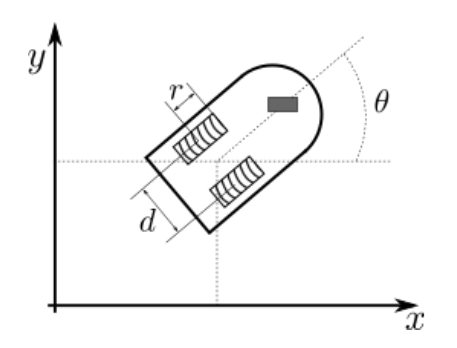
\includegraphics[scale=0.4]{other/differential_drive.png}
    \caption{Differential drive robot}
\end{figure}

The kinematic model of a differential drive vehicle is:

$$
\begin{cases}
    \dot{x} = \frac{\omega_r + \omega_l}{2} r \cos(\theta) \\
    \dot{y} = \frac{\omega_r + \omega_l}{2} r \sin(\theta) \\
    \dot{\theta} = \frac{\omega_r - \omega_l}{d} r \\
\end{cases}
$$

The linear and angular velocities of the vehicle are related to wheel velocities by the simple equations:

$$
\begin{cases}
    \omega_r = {\frac {v + \omega \cdot d/2}{r}} \\
    \omega_l = {\frac {v - \omega \cdot d/2}{r}}
\end{cases}
$$




%--------------------------------------------------------------------------------------------------------------
%                                               DWA OVERVIEW
%--------------------------------------------------------------------------------------------------------------

\section{DWA overview}

This section contains a brief overview of DWA as presented in the original
paper\footnote{\href{https://www.ri.cmu.edu/pub_files/pub1/fox_dieter_1997_1/fox_dieter_1997_1.pdf}
{D. Fox, W. Burgard, S. Thrun (1997) \textit{The Dynamic Window Approach to Collision Avoidance}}}.
Basically, it is an approach to perform collision avoidance in mobile robots, while dealing with the constraints
imposed by limited velocities and accelerations.\\

Given a certain goal point to be reached by the robot, DWA tries to find the optimal linear and angular velocities
to go there. This is mainly done in two steps: search space reduction and objective function optimization.


%------------------------------------------ SEARCH SPACE REDUCTION ------------------------------------------

\subsection{Search space reduction}

This approach consists in reducing the search space to those velocities which are reachable under the dynamic
constraints and are safe with respect to obstacles.

One of the core concepts of DWA is the so-called search space. It can be seen as a two-dimensional space where
each point represents a tuple $(v, \omega)$ of velocities, where $v$ is the linear velocity of the robot and
$\omega$ is the angular velocity.\\

An initial reduction of this space is obtained by searching only in circular trajectories of the robot.

In fact, at each time instant the velocities $(v, \omega)$ are considered constant for the next \textit{n}
time intervals making up the simulated trajectory. The search is repeated after each time interval.\\

The search space is further reduced by considering only all the admissible velocities, which correspond to
the velocities allowing the robot to stop before it reaches the closest obstacle.

Finally, given the limited accelerations of the robot, all the velocities that can't be reached within a short
time interval are left out too.\\


%-------------------------------------- OBJECTIVE FUNCTION OPTIMIZATION ---------------------------------------

\subsection{Objective function optimization}

The remaining velocities are fed into the following objective function to be maximized:
$$
G(v, \omega) = \sigma(\alpha \cdot heading(v, \omega)
+ \beta \cdot dist(v, \omega) + \gamma \cdot vel(v, \omega))
$$

This function trades off the following aspects:
\begin{itemize}
    \item \textit{heading}, which is a measure of progress towards the goal location;
    \item \textit{dist}, which is the distance to the closest obstacle on the trajectory;
    \item \textit{vel}, which is the forward velocity of the robot.\\
\end{itemize}

Each one of the three quantities above is multiplied to its own weight ($\alpha$, $\beta$, $\gamma$),
and the resulting quantity is passed to a smoothing function ($\sigma$).\\

At this point the tuple $(v, \omega)$ leading to the highest score is chosen and the robot picks those velocities.




%--------------------------------------------------------------------------------------------------------------
%                                                DWA IN ROS
%--------------------------------------------------------------------------------------------------------------

\section{DWA in ROS}


%------------------------------------------ FROM ROS WIKI ------------------------------------------

\subsection{From ROS wiki}

DWA is already implemented in ROS in the \texttt{dwa\_local\_planner}\footnote
{\href{https://wiki.ros.org/dwa\_local\_planner}{https://wiki.ros.org/dwa\_local\_planner}} package.\\

As stated in the ROS Wiki:
\begin{quote}
    ``This package provides a controller that drives a mobile base in the plane. This controller serves to connect the path planner to the robot. Using a map, the planner creates a kinematic trajectory for the robot to get from a start to a goal location. Along the way, the planner creates, at least locally around the robot, a value function, represented as a grid map. This value function encodes the costs of traversing through the grid cells. The controller's job is to use this value function to determine dx,dy,dtheta velocities to send to the robot.''
\end{quote}

This package is ought to be used as the planner for \texttt{move\_base}\footnote
{\href{https://wiki.ros.org/move\_base}{https://wiki.ros.org/move\_base}} (package providing an
implementation of an action that, given a goal in the world, will attempt to reach it with a mobile
base) within the navigation stack.\\

In the Wiki the following cost function to score each trajectory is presented:

\begin{tcolorbox}[enhanced,width=6in,center,size=fbox]

cost \textbf{=} path\_distance\_bias \textbf{*} (distance to path from the endpoint of the trajectory)\\
    \hspace*{4em}\textbf{+} goal\_distance\_bias \textbf{*}(distance to local goal from the endpoint of the trajectory)\\
    \hspace*{4em}\textbf{+} occdist\_scale \textbf{*} (maximum obstacle cost along the trajectory in obstacle cost (0-254))

\end{tcolorbox}

However, reading through the source code of the DWA ROS library, it is said that the above function is
\textit{``used for visualization only, total\_costs are not really total costs''}
\footnote{\href{https://docs.ros.org/en/melodic/api/dwa\_local\_planner/html/dwa\_\_planner\_8cpp\_source.html}
{https://docs.ros.org/en/melodic/api/dwa\_local\_planner/html/dwa\_\_planner\_8cpp\_source.html}}.
This is because ROS uses a slightly different cost function that will be described in the next paragraph.


%------------------------------------------ ROS LIBRARY SOURCE CODE ------------------------------------------

\subsection{ROS libray source code}

In order to use DWA standalone, it is possible to use the \texttt{DWAPlannerROS::computeVelocityCommands()} function
which leads to the following cascading function calls:\\
\begin{enumerate}

    \item \texttt{DWAPlannerROS::computeVelocityCommands()}\footnote
    {\href{https://docs.ros.org/en/melodic/api/dwa\_local\_planner/html/dwa\_\_planner\_\_ros\_8cpp\_source.html}
    {https://docs.ros.org/en/melodic/api/dwa\_local\_planner/html/dwa\_\_planner\_\_ros\_8cpp\_source.html}}
    called by \texttt{diffdrive\_traj\_ctrl.cpp} at line 78;

    \item \texttt{DWAPlannerROS::dwaComputeVelocityCommands()}\footnote
    {\href{https://docs.ros.org/en/melodic/api/dwa\_local\_planner/html/dwa\_\_planner\_\_ros\_8cpp\_source.html}
    {https://docs.ros.org/en/melodic/api/dwa\_local\_planner/html/dwa\_\_planner\_\_ros\_8cpp\_source.html}}
    called by function above at line 302;

    \item \texttt{DWAPlanner::findBestPath()}\footnote
    {\href{https://docs.ros.org/en/melodic/api/dwa\_local\_planner/html/dwa\_\_planner\_8cpp\_source.html}
    {https://docs.ros.org/en/melodic/api/dwa\_local\_planner/html/dwa\_\_planner\_8cpp\_source.html}}
    called by function above at line 209;

    \item \texttt{SimpleScoredSamplingPlanner::findBestTrajectory()}\footnote
    {\href{https://docs.ros.org/en/melodic/api/base\_local\_planner/html/simple\_\_scored\_\_sampling\_\_planner\_8cpp\_source.html}
    {https://docs.ros.org/en/melodic/api/base\_local\_planner/html/simple\_\_scored\_\_sampling\_\_planner\_8cpp\_source.html}}
    called by function above at line 317;

    \item \texttt{SimpleScoredSamplingPlanner::scoreTrajectory()}\footnote
    {\href{https://docs.ros.org/en/melodic/api/base\_local\_planner/html/simple\_\_scored\_\_sampling\_\_planner\_8cpp\_source.html}
    {https://docs.ros.org/en/melodic/api/base\_local\_planner/html/simple\_\_scored\_\_sampling\_\_planner\_8cpp\_source.html}}
    called by function above at line 105.\\

\end{enumerate}

At this point, \texttt{scoreTrajectory()} evaluates the different cost elements of a single trajectory in order to
give it a score. This score will be used to determine the best trajectory among all the evaluated ones.

Each cost element is an instance of the abstract \texttt{base\_local\_planner::TrajectoryCostFunction} class,
and takes into account a different aspect of the trajectory.\\

These elements are contained in a \texttt{std::vector<TrajectoryCostFunction*>} vector and, in the case
of DWA, they are 7 in total:

\begin{itemize}
    \item \texttt{base\_local\_planner::OscillationCostFunction oscillation\_costs\_},
            which penalizes trajectories where the robot oscillates;
    \item \texttt{base\_local\_planner::ObstacleCostFunction obstacle\_costs\_},
            which penalizes trajectories where the robot occupies illegal positions with its footprint;
    \item \texttt{base\_local\_planner::MapGridCostFunction goal\_front\_costs\_},
            which prefers  trajectories that make the nose go towards (local) nose goal;
    \item \texttt{base\_local\_planner::MapGridCostFunction alignment\_costs\_},
            which prefers trajectories that keep the robot nose on nose path;
    \item \texttt{base\_local\_planner::MapGridCostFunction path\_costs\_},
            which prefers trajectories on global path;
    \item \texttt{base\_local\_planner::MapGridCostFunction goal\_costs\_},
            which prefers trajectories that go towards (local) goal;
    \item \texttt{base\_local\_planner::TwirlingCostFunction twirling\_costs\_},
            which prefers trajectories that don't spin.\\
\end{itemize}

The final score of each trajectory is then computed as the sum of all the cost elements above.\\

It is worth mentioning that the trajectories evaluated by DWA are obtained through the

\texttt{base\_local\_planner::SimpleTrajectoryGenerator}\footnote
{\href{https://docs.ros.org/en/melodic/api/base\_local\_planner/html/classbase\_\_local\_\_planner\_1\_1SimpleTrajectoryGenerator.html}
{https://docs.ros.org/en/melodic/api/base\_local\_planner/html/classbase\_\_local\_\_planner\_1\_1SimpleTrajectoryGenerator.html}}
class, which generates trajectories by performing an equi-distant discretization of the velocities that
the robot can assume.\\




%--------------------------------------------------------------------------------------------------------------
%                                        TRAJECTORY TRACKING CONTROLLER
%--------------------------------------------------------------------------------------------------------------

\section{Trajectory tracking controller}


%---------------------------------------- UNICYCLE MODEL CONTROL ----------------------------------------

\subsection{Unicycle model control}

When designing the controller it is possible to work on the unicycle (thus not differential) model, for simplicity:

$$
\begin{cases}
    \dot{x} = v \cdot \cos(\theta) \\
    \dot{y} = v \cdot \sin(\theta) \\
    \dot{\theta} = \omega \\
\end{cases}
$$

In fact, the differential model can be easily reduced to the unicycle one with the transformations:

$$
\begin{cases}
    v = {\frac {\omega_r + \omega_l}{2} r} \\
    \omega = {\frac {\omega_r - \omega_l}{2} r} \\
\end{cases}
$$

With this simple substitution the differential model is obtained:

$$
\begin{cases}
    \dot{x} = \frac{\omega_r + \omega_l}{2} r \cos(\theta) \\
    \dot{y} = \frac{\omega_r + \omega_l}{2} r \sin(\theta) \\
    \dot{\theta} = \frac{\omega_r - \omega_l}{d} r \\
\end{cases}
$$

Going back to the unicycle, which is simpler to work on, we must consider a point P on the robot chassis for
control purposes, since the contact point of the wheel is affected by a nonholonomic constraint.\\

\begin{figure}[H]
    \centering
    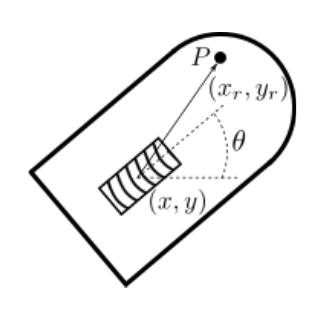
\includegraphics[scale=0.5]{other/point_p.png}
    \caption{Point P on the robot chassis.}
\end{figure}

Therefore all the goal points that the robot must reach will be translated into goals for the point P,
as explained in the next few paragraphs.


%---------------------------------------- CONTROLLER'S ARCHITECTURE ----------------------------------------

\subsection{Controller's architecture}

The developed controller works by taking only the reference points (making up the full trajectory),
and then computing everything else on its own.\\

A comprehensive schematic representation of the whole controller is shown in the diagram below:\\

\begin{figure}[H]
    \centering
    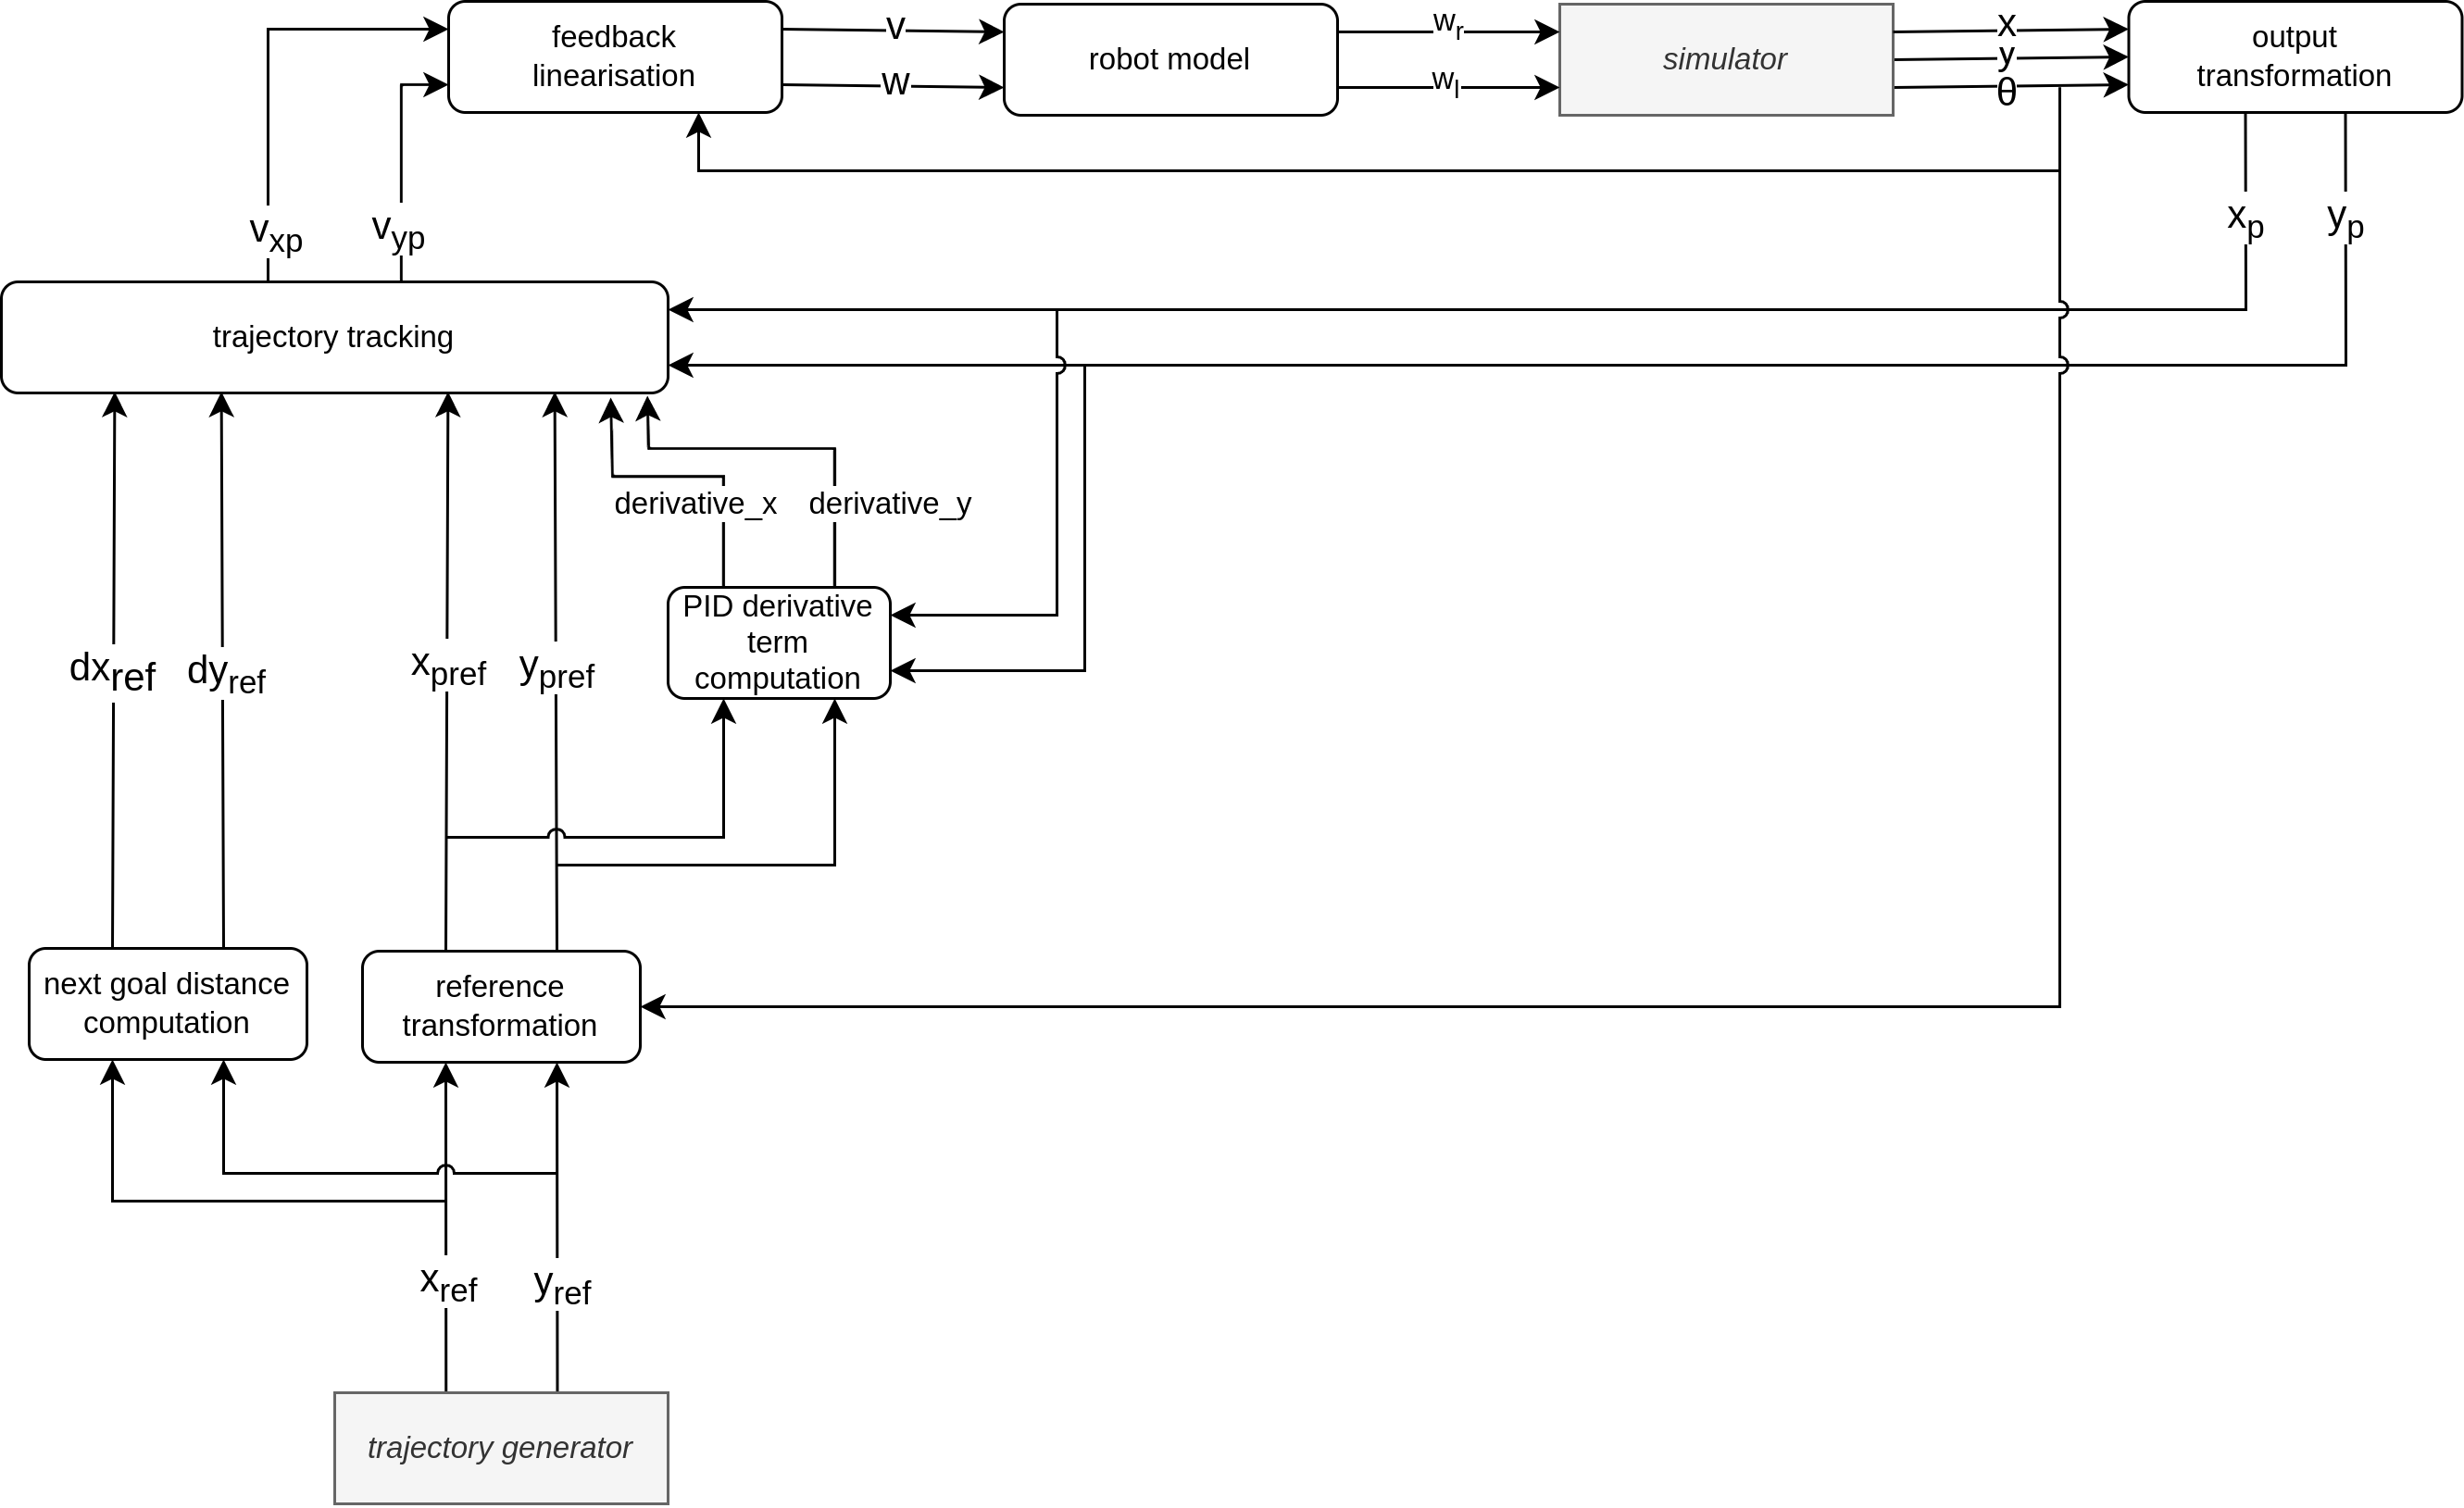
\includegraphics[scale=0.17]{other/custom_controller.png}
    \caption{Scheme of the custom controller.}
\end{figure}

Let's break down the operations performed by each one of the blocks in the diagram.\\

The ``trajectory tracking'' block computes the linear velocity of point P:
$$v_{Px} = dx_{ref} + K_p \cdot error_{Px} + K_i \cdot error_{Px} \cdot RunPeriod + K_d \cdot derivative\_x$$
$$v_{Py} = dy_{ref} + K_p \cdot error_{Py} + K_i \cdot error_{Px} \cdot RunPeriod + K_d \cdot derivative\_y$$ \\

The ``feedback linearisation'' block computes the linear and angular velocities of the robot:
$$v = v_{Px} \cdot \cos(\theta)  +  v_{Py} \cdot \sin(\theta)$$
$$\omega = \frac {v_{Py} \cdot \cos(\theta)  - v_{Px} \cdot \sin(\theta)}{P\_dist}$$ \\

The ``robot model'' block computes the angular velocities of the wheels:
$$\omega_r = \frac {v + \omega \cdot \frac{d}{2}}{r}$$
$$\omega_l = \frac {v - \omega \cdot \frac{d}{2}}{r}$$ \\

The ``output transformation'' block computes the new position of point P:
$$x_P = x + P\_dist \cdot \cos(\theta)$$
$$y_P = y + P\_dist \cdot \sin(\theta)$$ \\

The ``next goal distance computation'' block computes the distance between the old goal and the new goal:
$$dx_{ref} = x_{ref,t+1} - x_{ref,t} $$
$$dy_{ref} = y_{ref,t+1} - y_{ref,t} $$ \\

The ``reference transformation'' block computes the reference position for point P (goal for point P):
$$x_{Pref} = x_{ref} + P\_dist \cdot \cos(\theta)$$
$$y_{Pref} = y_{ref} + P\_dist \cdot \sin(\theta)$$ \\

The ``PID derivative term computation'' block computes the derivative term for the PID controller:
$$error\_x = x_{Pref} - x_P$$
$$error\_y = y_{Pref} - y_P$$
$$derivative\_x = \frac {error\_x - error\_x_{prev}}{RunPeriod}$$
$$derivative\_y = \frac {error\_y - error\_y_{prev}}{RunPeriod}$$ \\

In the scheme there are also two blocks that are outside of the controller:
\begin{itemize}
    \item the ``simulator'' block, which updates the pose of the robot given the angular velocities of the wheels;
    \item the ``trajectory generator'' block, which creates a vector of reference positions for the robot
            (goals for the center of the robot).
\end{itemize}




%--------------------------------------------------------------------------------------------------------------
%                                           SETUP OF THE EXPERIMENT
%--------------------------------------------------------------------------------------------------------------

\section{Setup of the experiment}


%------------------------------------------ THE ROBOT ------------------------------------------

\subsection{The robot}

The differential drive robot that has been chosen for the simulation is characterized by the following
two dimensions, which are specified as YAML parameters in the code:
\begin{itemize}
    \item \texttt{d} = 15 cm, which is the distance between the two wheels;
    \item \texttt{r} = 3 cm, which is the radius of the two wheels.\\
\end{itemize}

The precise footprint of the robot is a pentagon, just for convenience, so that it is easy to determine its
orientation when looking at it in \textit{Rviz}.
However, this is a minor detail since it has no influence on the robot's behavior.


%------------------------------------------ THE MAP ------------------------------------------

\subsection{The map}

The map is a component required by DWA to be able to work. Differently from the usual setting in which
DWA is used, three main differences characterize this experiment:
\begin{itemize}
    \item there are no obstacles in the map, neither fixed nor moving, and the robot does not have any sensor;
    \item the robot must follow a predefined trajectory, no global plan has to be computed.\\
\end{itemize}

As a consequence, we don't need both the local map and the global map, but only the global one.

Moreover, this map needs to be empty since it is static and obstacles-free, so it can be
generated starting from a totally white image.


%------------------------------------------ THE TRAJECTORY ------------------------------------------

\subsection{The trajectory}

The robot must follow a precise trajectory: an eight-shaped trajectory with a dimension of 2 x 1 meters,
which is used to perform all benchmarks.\\

In order to make DWA compute the velocities of the robot, a goal is required.
This means that the complete trajectory needs to be "discretized" in multiple points, each one representing a goal.
These points are then passed to DWA one at a time and set as the current goal.
Once a point is reached the next one is set as the new goal.
A more-detailed explanation can be found in the following sections.




%--------------------------------------------------------------------------------------------------------------
%                                           IMPLEMENTATION
%--------------------------------------------------------------------------------------------------------------

\section{Implementation}


%------------------------------------------ ARCHITECTURE OVERVIEW ------------------------------------------

\subsection{Architecture overview}

The code used for this experiment is divided into three packages: one simulator (\texttt{diffdrive\_kin\_sim})
and two controllers (\texttt{diffdrive\_kin\_ctrl} and \texttt{diffdrive\_dwa\_ctrl}).

The two controllers, one implementing a trajectory tracking law and the other implementing DWA,
are interchangeable and are meant to always be used together with the simulator, one at a time.

\subsection{Services}

A ROS service named \texttt{generate\_desired\_path\_service}, implemented in \texttt{eight\_traj\_gen.cpp}, is used to generate the eight-shaped
trajectory that the robot must follow.\\

First, the two vectors contained in the \texttt{GenerateDesiredPathService.srv} message are populated
with the coordinates of all the points of the trajectory.

Then, as soon as the service is called during the initialization (\texttt{Prepare()} function) of both
controllers, the complete trajectory is made available also to them.


%------------------------------------------ NODES ------------------------------------------

\subsection{Nodes}

\subsubsection{\texttt{diffdrive\_kin\_sim\_node}}

This node is subscribed to the \texttt{/robot\_input} topic and reads the angular velocities
of the wheels.

Given those it simulates the movement of the robot and publishes the new position on both
\texttt{/robot\_state} and \texttt{/odom} topics.
These two topics are kept separated in order to accommodate both controllers.\\

The actual simulator is an object of the \texttt{diffdrive\_kin\_ode} class, which is initialized with
\begin{lstlisting}
simulator = new diffdrive_kin_ode(dt);
\end{lstlisting}

and contains the integration logic to update the robot pose.

\subsubsection{\texttt{diffdrive\_kin\_trajctrl\_node}}

This node is dedicated to computing the angular velocities of the two wheels given the current position
of the robot and its next point in the trajectory, using a custom trajectory tracking controller.\\

During the initialization phase it queries the \texttt{generate\_desired\_path\_service} service and
stores the complete trajectory.
Then, every time a message is published on the \texttt{/robot\_state} topic this node updates its
internal values of the robot pose.\\

The \texttt{PeriodicTask()} that gets executed uses a PID controller and a linearisation law (implemented
in the \texttt{diffdrive\_kin\_fblin} class) to compute both the linear and the angular velocities
$(v, \omega)$ of the robot.

As a last step, since the simulated robot is a differential drive one, the angular velocities of
the two wheels are computed starting from the $(v, \omega)$ above, and the new results are published
on the \texttt{/robot\_input} and \texttt{/controller\_state} topics.

\subsubsection{\texttt{diffdrive\_dwa\_trajctrl\_node}}

Similarly to the custom controller explained before, this node computes the angular velocities of
the two wheels.\\

This node is used to interface the DWA library in ROS with the custom simulator (in order to compute
the angular velocities of the two wheels, just like the previous controller).
This is due to the fact that natively DWA is used inside ROS Navigation Stack, thus it expects
an odometry source and a costmap.\\

\begin{figure}[H]
    \centering
    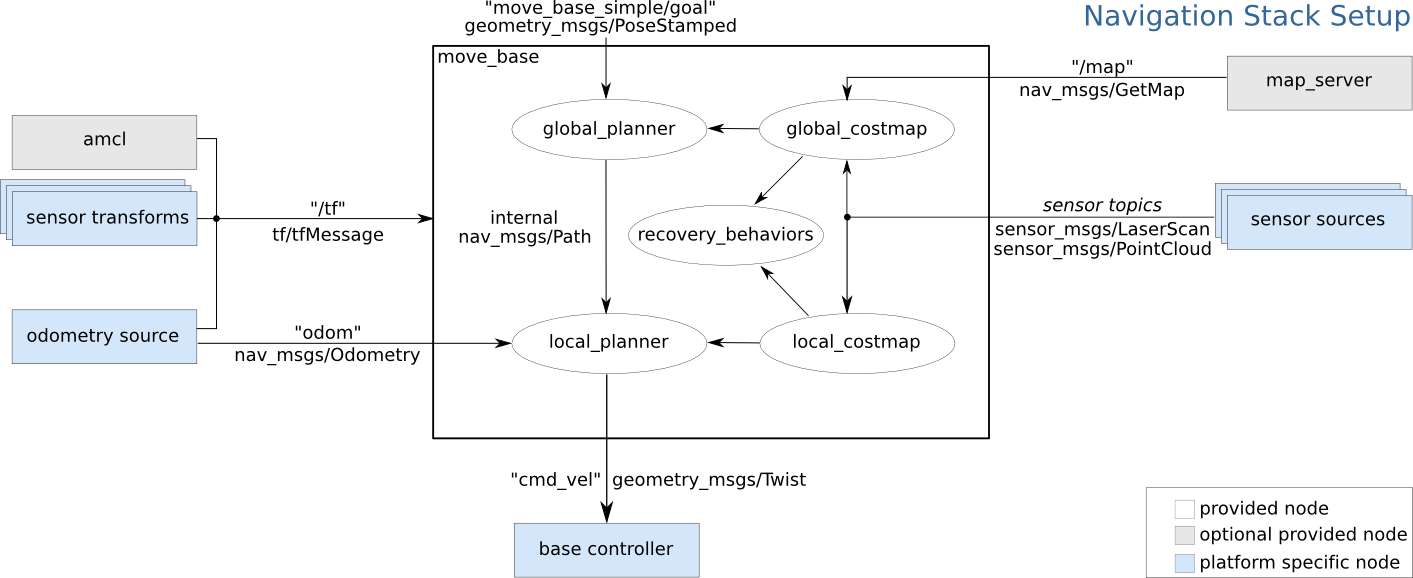
\includegraphics[scale=0.4]{other/navigation_stack.png}
    \caption{ROS Navigation Stack.}
\end{figure}

In this specific implementation of this experiment only a global costmap and a planner (DWA) are used,
for the reasons explained before.\\

During the initialization phase the service is queried.
The trajectory is received and one point every \texttt{skipped\_goals} is set as the new plan for DWA
(note: the plan here is made of just one point).

Once the plan is set, the DWA controller tries to reach the new goal position by computing the necessary
pair of $(v, \omega)$ velocities. As soon as the goal is reached with a certain tolerance, the next point
in the trajectory is set as the new goal.\\

Lastly, the $(\omega_r,\omega_l)$ velocities of the two wheels are computed and published on the
\texttt{/robot\_input} and

\texttt{/controller\_state} topics.\\

The implementation of DWA and all the functions that have been used is provided by the following
two files in the ROS library:
\begin{itemize}
    \item \href{https://docs.ros.org/en/melodic/api/dwa\_local\_planner/html/dwa\_\_planner\_8cpp\_source.html}
            {\texttt{dwa\_local\_planner/dwa\_planner.cpp}}
    \item \href{https://docs.ros.org/en/melodic/api/dwa\_local\_planner/html/dwa\_\_planner\_\_ros\_8cpp\_source.html}
            {\texttt{dwa\_local\_planner/dwa\_planner\_ros.cpp}}
\end{itemize}

\subsubsection{\texttt{odom\_to\_baselink\_tf\_node}}

This is a very simple node. It links the \texttt{odom} and the \texttt{base\_link}
coordinate frames through a dynamic tf, since the robot footprint (which is in the \texttt{base\_link}
frame) must be somehow related to the environment (the robot starts moving in the \texttt{odom} frame).


%------------------------------------------ FRAMES ------------------------------------------

\subsection{Frames}

Here is a list of all the frames, with a short description:
\begin{itemize}
    \item \texttt{map}, which is the coordinate system where the empty map (provided by the map server) is;
    \item \texttt{odom}, which represents the global reference system, whose origin matches the one of
            the \texttt{map} frame in this particular case;
    \item \texttt{base\_link}, which represents reference system moving around together with the robot.
\end{itemize}

\begin{figure}[H]
    \centering
    \subfloat[Frames of the custom controller.]{
        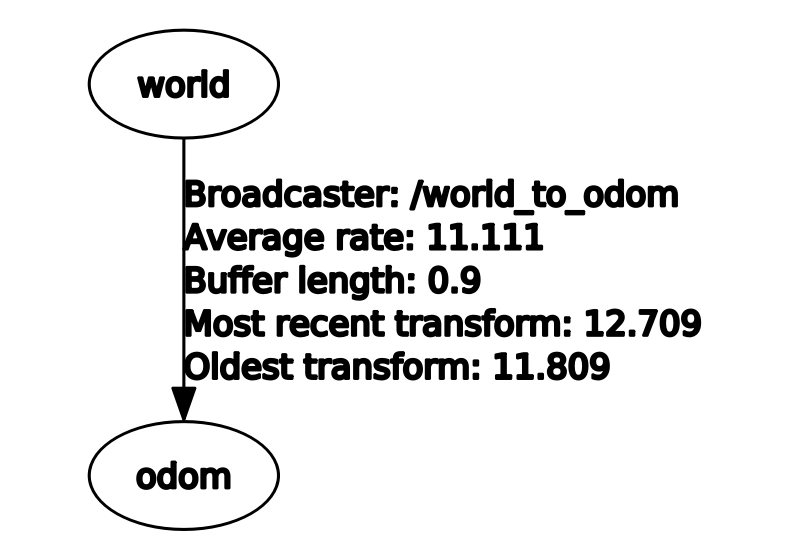
\includegraphics[scale=0.28]{ros_tools/rqttftree_custom.png}
    }
    \subfloat[Frames of DWA standalone.]{
        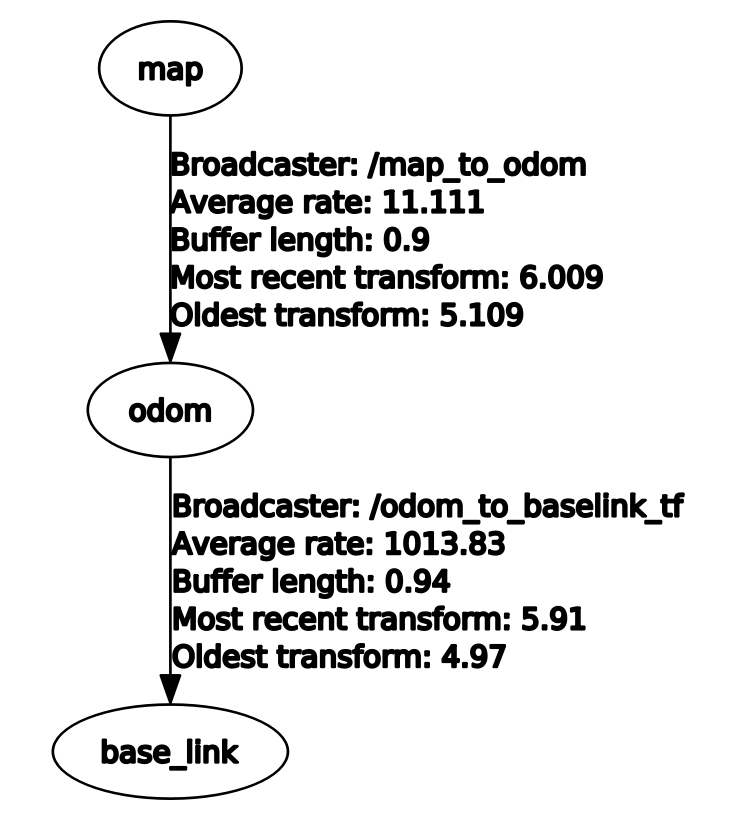
\includegraphics[scale=0.26]{ros_tools/rqttftree_dwa.png}
    }
    \caption[]{Frames (obtained with \texttt{rqt\_tf\_tree}) of the two approaches.}
\end{figure}


%------------------------------------------ TOPICS ------------------------------------------

\subsection{Topics}

Here is a list of the topics used by nodes for publishing or subscribing, with a short description :\\

\begin{itemize}

    \item \texttt{/clock}, used to synchronize all the nodes in the simulation;

    \item \texttt{/odom}, used to pass the odometry information of the robot to DWA;
        \begin{itemize}
            \item publishers:
                \begin{itemize}
                    \item \texttt{diffdrive\_kin\_sim}
                \end{itemize}
            \item subscribers:
                \begin{itemize}
                    \item \texttt{odom\_to\_baselink\_tf}
                \end{itemize}
        \end{itemize}

    \item \texttt{/robot\_state}, used to communicate the odometry information of the robot to the custom controller;
        \begin{itemize}
            \item publishers:
                \begin{itemize}
                    \item \texttt{diffdrive\_kin\_sim}
                \end{itemize}
            \item subscribers:
                \begin{itemize}
                    \item \texttt{diffdrive\_kin\_trajctrl}
                \end{itemize}
        \end{itemize}

    \item \texttt{/controller\_state}, used to publish the details about the controller for visualization purposes;
        \begin{itemize}
            \item publishers:
                \begin{itemize}
                    \item \texttt{diffdrive\_kin\_trajctrl}
                    \item \texttt{diffdrive\_dwa\_trajctrl}
                \end{itemize}
            \item subscribers:
                \begin{itemize}
                    \item \textit{none}
                \end{itemize}
        \end{itemize}

    \item \texttt{/robot\_input}, used to communicate $(\omega_r,\omega_l)$ computed by the controllers;
        \begin{itemize}
            \item publishers:
                \begin{itemize}
                    \item \texttt{diffdrive\_kin\_trajctrl}
                    \item \texttt{diffdrive\_dwa\_trajctrl}
                \end{itemize}
            \item subscribers:
                \begin{itemize}
                    \item \texttt{diffdrive\_kin\_sim}
                \end{itemize}
        \end{itemize}

\end{itemize}


%------------------------------------------ LAUNCH FILES ------------------------------------------

\subsection{Launch files}

Here is a list of the two launch files, with a short description:\\
\begin{itemize}
    \item \texttt{diffdrive\_kin\_trajctrl.launch}, used to simulate the behavior of the robot
            with the custom controller by starting the following nodes:
        \begin{itemize}
            \item \texttt{diffdrive\_kin\_sim} (simulator)
            \item \texttt{diffdrive\_kin\_trajctrl} (trajectory tracking controller)
            \item \texttt{eight\_traj\_gen} (trajectory generator)
            \item \texttt{world\_to\_odom} (static tf linking \texttt{world} and \texttt{odom} frames)
            \item \texttt{odom\_visualizer} (\textit{Rviz} node to visualize real-time data)\\
        \end{itemize}

    \item \texttt{diffdrive\_dwa\_trajctrl.launch}, used to simulate the behavior of the robot
            with DWA by starting the following nodes:
        \begin{itemize}
            \item \texttt{diffdrive\_kin\_sim} (simulator)
            \item \texttt{diffdrive\_dwa\_trajctrl} (DWA)
            \item \texttt{eight\_traj\_gen} (trajectory generator)
            \item \texttt{odom\_to\_baselink\_tf} (dynamic tf linking \texttt{odom} and \texttt{base\_link} frames)
            \item \texttt{map\_node} (\textit{map\_server} node used to provide the map)
            \item \texttt{map\_to\_odom} (static tf linking \texttt{map} and \texttt{odom} frames)
            \item \texttt{odom\_visualizer} (\textit{Rviz} node to visualize data)
        \end{itemize}
\end{itemize}

\begin{figure}[H]
    \centering
    \subfloat[Architecture of the custom controller.]{
        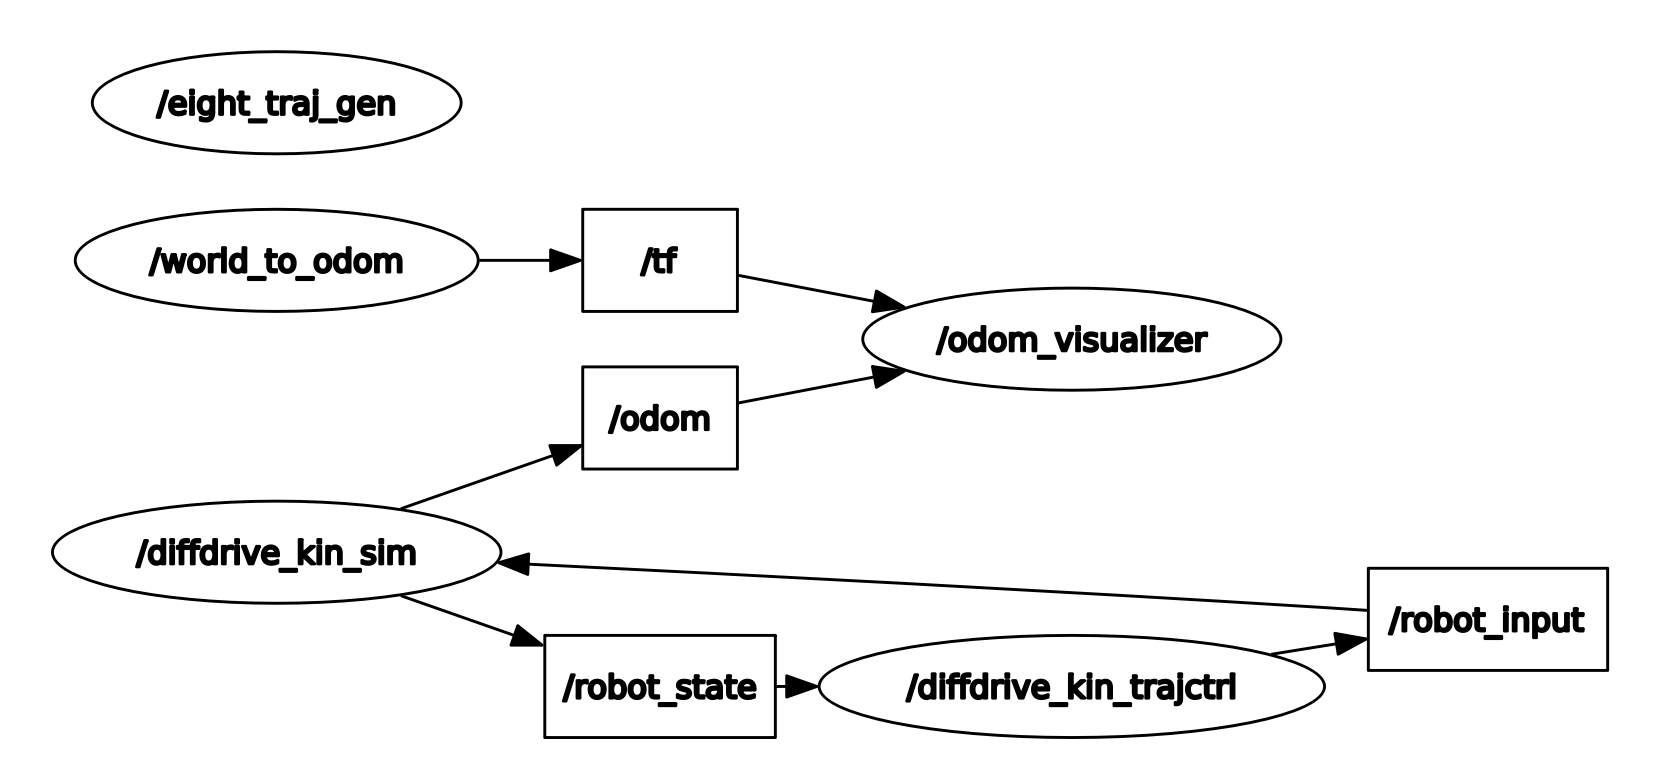
\includegraphics[scale=0.16]{ros_tools/rqtgraph_custom.png}
    }
    \quad
    \subfloat[Architecture of DWA standalone.]{
        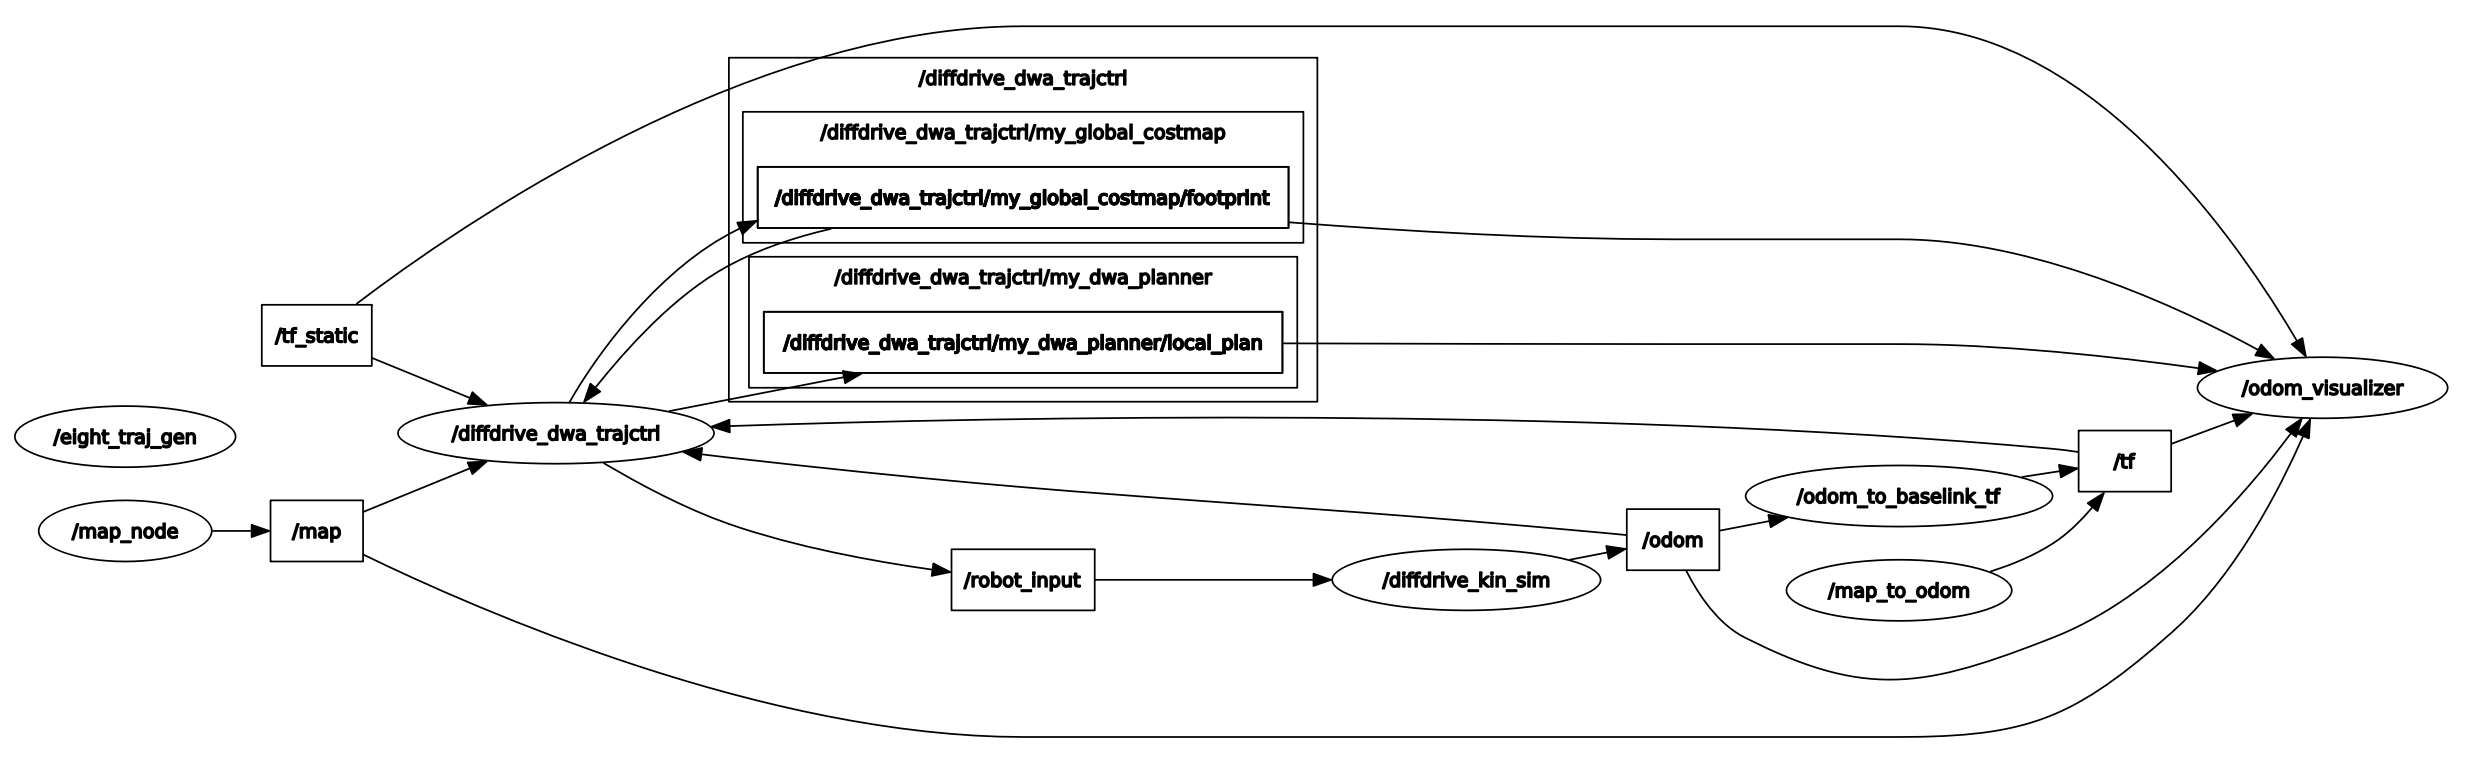
\includegraphics[scale=0.25]{ros_tools/rqtgraph_dwa.png}
    }
    \caption[]{Architecture (obtained with \texttt{rqt\_graph}) of the two approaches.}
\end{figure}




%--------------------------------------------------------------------------------------------------------------
%                                               PARAMETERS
%--------------------------------------------------------------------------------------------------------------

\section{Parameters}


%------------------------------------------ LIST OF PARAMETERS ------------------------------------------

\subsection{List of parameters}

Parameters have a crucial role for the correct functioning of the nodes introduced above.
Some are strictly required for the implementation to be started, others can be tuned to slightly
change the behavior of the robot when following the trajectory.\\

In this section the most relevant ones are listed, with a short description:\\
\begin{itemize}

    \item \texttt{diffdrive\_kin\_sim/config/diffdrive\_kin\_sim.yaml}:
        \begin{itemize}
            \item \texttt{d}, distance between the two wheels;
            \item \texttt{r}, radius of the two wheels.\\
        \end{itemize}

    \item \texttt{diffdrive\_kin\_trajctrl/config/eight\_traj.yaml}:
        \begin{itemize}
            \item \texttt{a}, amplitude of the eight-shaped trajectory;
            \item \texttt{w}, ratio $\frac{2 \cdot \pi }{T}$ where $T$ is the time duration of each lap;
            \item \texttt{trajectory\_length}, length of the eight-shaped trajectory;
            \item \texttt{increment\_step}, increment step when discretizing the trajectory.\\
        \end{itemize}

    \item \texttt{diffdrive\_kin\_trajctrl/config/diffdrive\_kin\_trajctrl.yaml}:
        \begin{itemize}
            \item \texttt{Kp}, proportional gain of the PID controller;
            \item \texttt{Ki}, integral gain of the PID controller;
            \item \texttt{Kd}, derivative gain of the PID controller.\\
        \end{itemize}

    \item \texttt{diffdrive\_dwa\_trajctrl/config/diffdrive\_dwa\_trajctrl.yaml}:
        \begin{itemize}
            \item \texttt{skipped\_goals}, number of points to skip when feeding the trajectory to DWA.\\
        \end{itemize}

    \item \texttt{diffdrive\_dwa\_trajctrl/config/dwa\_planner\_params.yaml}:
        \begin{itemize}
            \item \texttt{min\_vel\_y}, minimum linear velocity along the y-axis;
            \item \texttt{max\_vel\_y}, maximum linear velocity along the y-axis;
            \item \texttt{min\_vel\_x}, minimum linear velocity along the x-axis;
            \item \texttt{max\_vel\_x}, maximum linear velocity along the x-axis;
            \item \texttt{acc\_lim\_theta}, maximum angular acceleration;
            \item \texttt{vth\_samples}, number of uniformly-sampled values of $\omega$ that DWA considers when simulating;
            \item \texttt{vx\_samples}, number of uniformly-sampled values of $v$ that DWA considers when simulating;
            \item \texttt{path\_distance\_bias}, weighting for how much the controller should stay close to the given path;
            \item \texttt{goal\_distance\_bias}, weighting for how much the controller should attempt to reach its local goal;
            \item \texttt{xy\_goal\_tolerance}, tolerance (in meters) in the x \& y distance when reaching a goal;
            \item \texttt{yaw\_goal\_tolerance}, tolerance (in radians) in yaw/rotation when reaching a goal.\\
        \end{itemize}

\end{itemize}


%------------------------------------------ PARAMETERS TUNING ------------------------------------------

\subsection{Parameters tuning}

\subsubsection{Eight-shaped trajectory}

An eight-shaped trajectory can be be described with the following analytical equations:
$$
\begin{cases}
    x = \texttt{a} \cdot \sin (\texttt{w} \cdot t)\\
    y = \texttt{a} \cdot \sin (\texttt{w} \cdot t)\cdot \cos (\texttt{w} \cdot t)\\
\end{cases}
$$

In the equations above it is possible to tune two parameters: \texttt{a} and \texttt{w}.
In the presented implementation they are set to \texttt{a} = 1 and \texttt{w} = 1.\\

\newpage

Here is what happens when \texttt{a} is increased (the eight-shape becomes larger, look at the scale):

\begin{figure}[H]
    \centering
    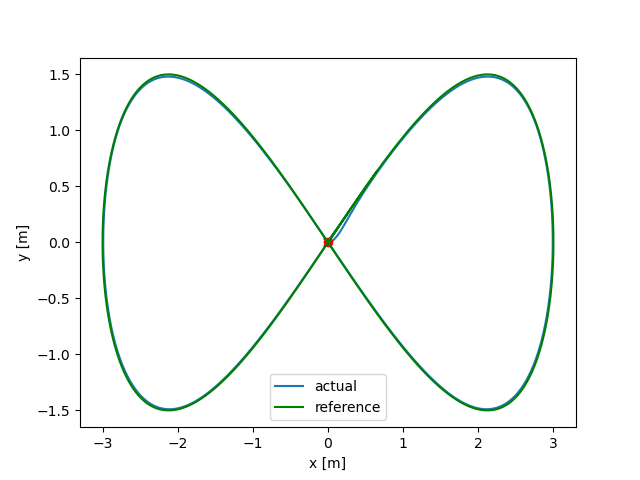
\includegraphics[scale=0.5]{different_params/custom_a3/Trajectory.png}
    \caption{Trajectory when \texttt{a = 3.0}.}
\end{figure}

\subsubsection{Custom controller}

The custom controller is a trajectory tracking one composed of an inner linearisation law and
an outer tracking law.
The outer tracking law is based on a PID controller with tunable parameters: $K_p$, $K_i$, $K_d$.\\

The step response when using a PID controller is computed as follows:
$$
u(t)=K_{\text{p}}e(t)+K_{\text{i}}\int _{0}^{t}e(\tau )\,\mathrm {d} \tau +K_{\text{d}}{\frac {\mathrm {d} e(t)}{\mathrm {d} t}}
$$\\

\begin{figure}[H]
    \centering
    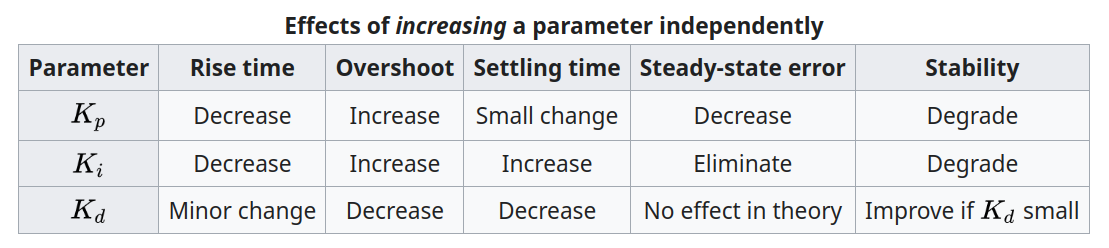
\includegraphics[scale=0.4]{other/PID_parameters_description.png}
    \caption{PID parameters tuning.}
\end{figure}

Various tests have been carried out to achieve the optimal behavior, in particular to minimize
the overshoot and the settling time while keeping an overall good stability in the PID response.\\

In the presented implementation they are set to $K_p = 0.8$, $K_i = 0.8$, $K_d = 0$.\\

\newpage

Here are two examples of poor performance when the PID parameters are not correctly tuned:

\begin{figure}[H]
    \centering
    \subfloat[Trajectory.]{
        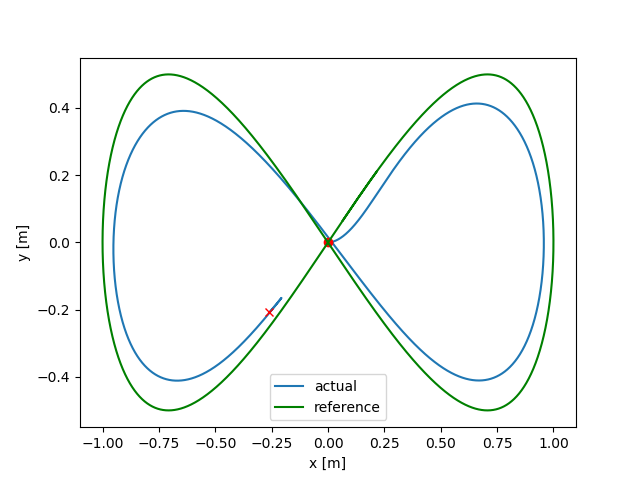
\includegraphics[scale=0.5]{different_params/custom_kp02/Trajectory.png}
    }
    \subfloat[Linear and angular velocities.]{
        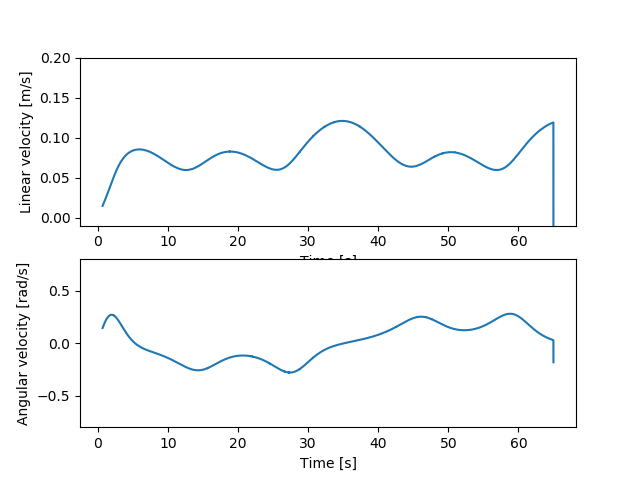
\includegraphics[scale=0.5]{different_params/custom_kp02/Linear_and_Angular_Velocities.png}
    }
    \caption[]{Behavior with $K_p=0.2, K_i=0.8, K_d=0.0$.}
\end{figure}

\begin{figure}[H]
    \centering
    \subfloat[Trajectory.]{
        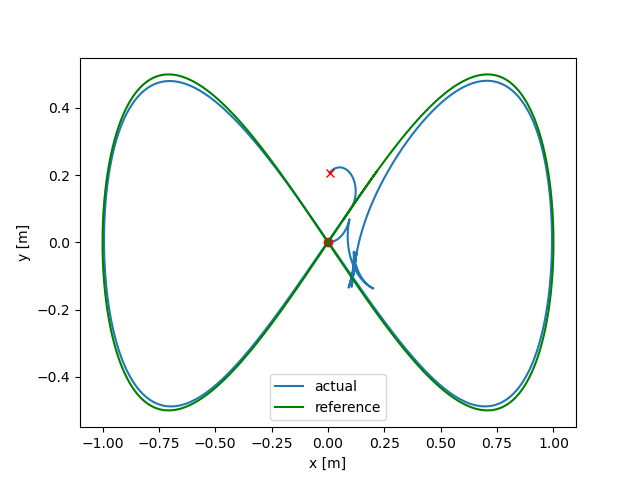
\includegraphics[scale=0.5]{different_params/custom_ki32kd10/Trajectory.png}
    }
    \subfloat[Linear and angular velocities.]{
        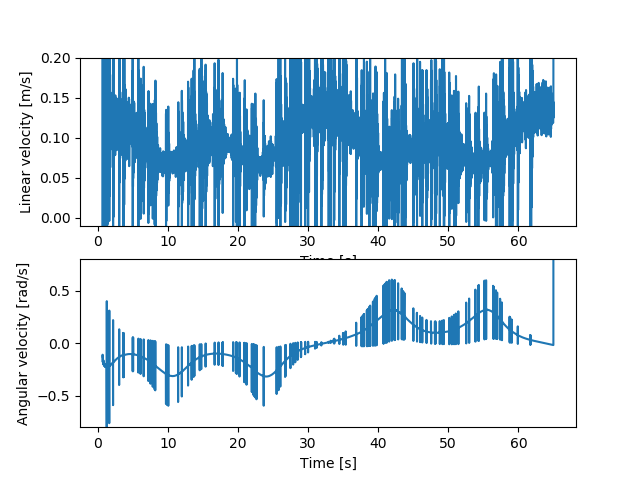
\includegraphics[scale=0.5]{different_params/custom_ki32kd10/Linear_and_Angular_Velocities.png}
    }
    \caption[]{Behavior with $K_p=0.8, K_i=3.2, K_d=1.0$.}
\end{figure}

\subsubsection{DWA}

When the trajectory is generated, the eight shape is discretized over numerous points.

Due to their large number, they are very close to each other. This makes the robot misbehave as soon as
a new goal is set in DWA: the distance between two consecutive goals must be higher.
For this reason it is best to skip some of the points in the trajectory.

This is accomplished through the \texttt{skipped\_goals} parameters, which is set to 15.\\

\newpage

If \texttt{skipped\_goals = 0} is set, then the number of spikes in the velocities of the robot increases:
\begin{figure}[H]
    \centering
    \subfloat[Trajectory.]{
        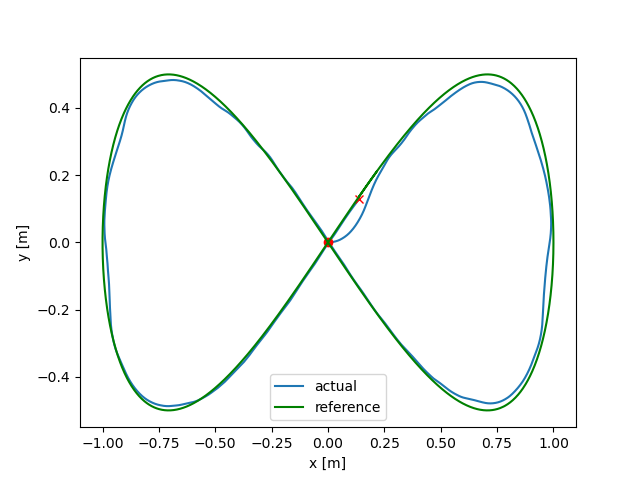
\includegraphics[scale=0.44]{different_params/dwa_skippedgoals0/Trajectory.png}
    }
    \quad
    \subfloat[Position Error.]{
        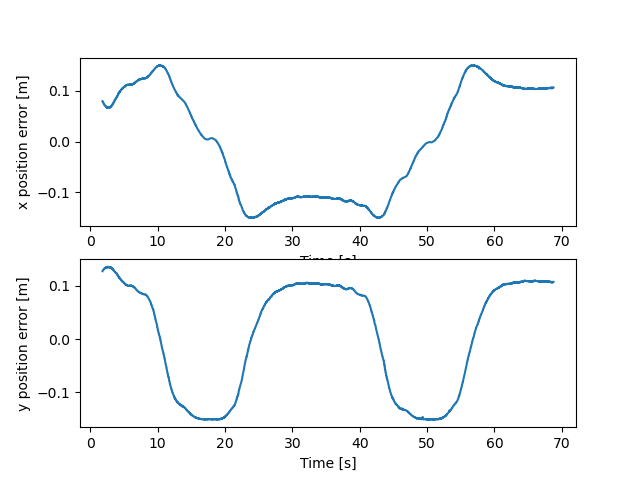
\includegraphics[scale=0.35]{different_params/dwa_skippedgoals0/Position_Error.png}
    }
    \subfloat[Linear and angular velocities.]{
        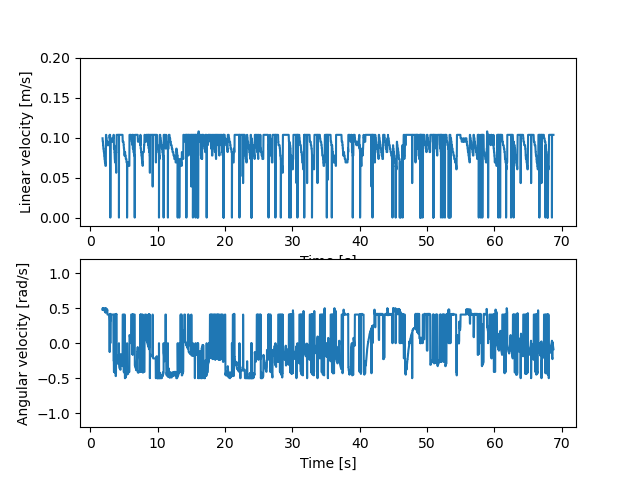
\includegraphics[scale=0.35]{different_params/dwa_skippedgoals0/Linear_and_Angular_Velocities.png}
    }
    \caption[]{Behavior with \texttt{skipped\_goals = 0}.}
\end{figure}

%\newpage

If instead \texttt{skipped\_goals = 150} is set, then the error in the position while following the trajectory increases:
\begin{figure}[H]
    \centering
    \subfloat[Trajectory.]{
        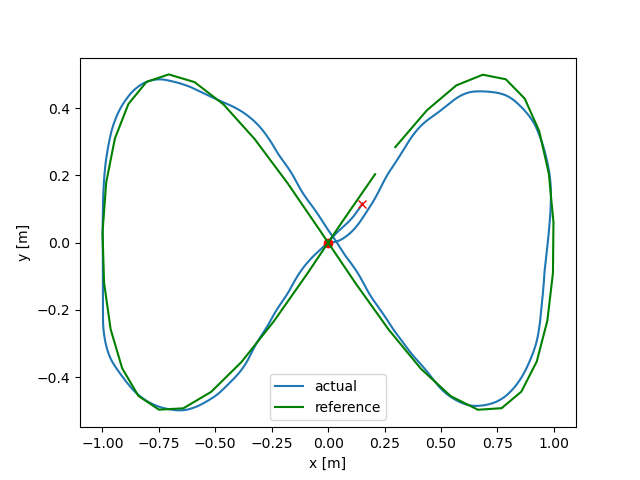
\includegraphics[scale=0.44]{different_params/dwa_skippedgoals150/Trajectory.png}
    }
    \quad
    \subfloat[Position Error.]{
        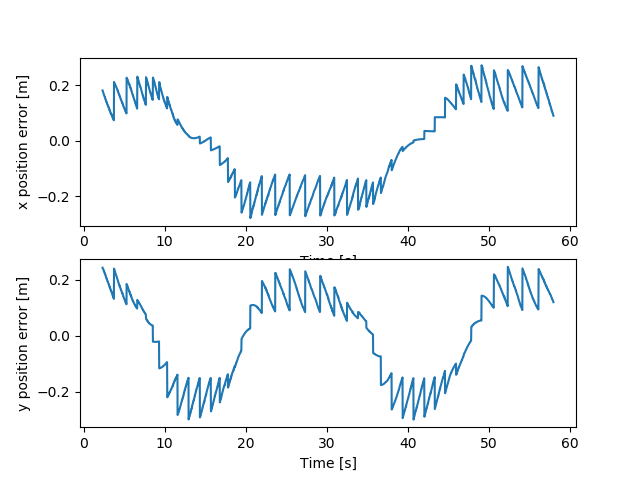
\includegraphics[scale=0.35]{different_params/dwa_skippedgoals150/Position_Error.png}
    }
    \subfloat[Linear and angular velocities.]{
        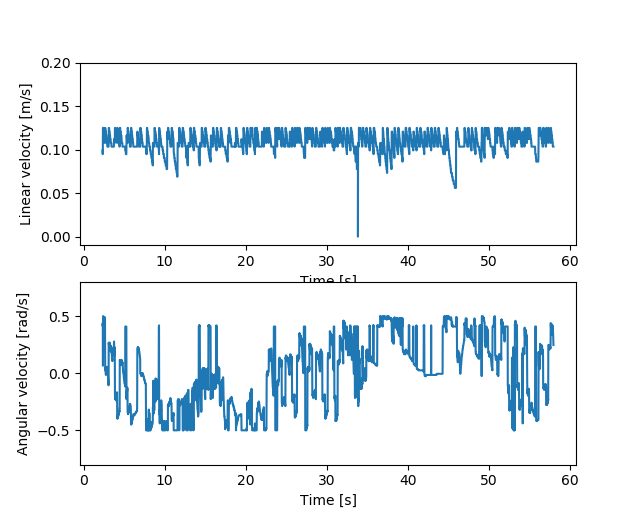
\includegraphics[scale=0.35]{different_params/dwa_skippedgoals150/Linear_and_Angular_Velocities.png}
    }
    \caption[]{Behavior with \texttt{skipped\_goals = 150}.}
\end{figure}

Since the robot to be simulated is a differential drive one, the following parameters must be set:
\begin{itemize}
    \item \texttt{min\_vel\_y} = 0 and \texttt{max\_vel\_y} = 0, to forbid lateral movement along the y-axis;
    \item \texttt{min\_vel\_x} = 0, to forbid backward movement along the x-axis.\\
\end{itemize}

Another parameter related to the constraints on the movement of the robot is \texttt{acc\_lim\_theta}.
To achieve the best trade-off betweeen the ability to correctly follow the trajectory and the realistic
constraints on the steering capabilities of the robot, the chosen value for it is 10.\\

Since DWA discretely samples in the robot's control space, parameters \texttt{vth\_samples}
and \texttt{vx\_samples} play a key role in allowing a finer grained choice of velocities.
To achieve the best trade-off betweeen a wide choice of possible $(v,\omega)$ and the computational effort
needed to perform the simulation, the optimal values have been found to be \texttt{vth\_samples = 100}
and \texttt{vx\_samples = 30}.\\

Finally, DWA provides a certain tolerance within which the goal is considered to be reached.
In particular this can be done through two parameters \texttt{yaw\_goal\_tolerance} and \texttt{xy\_goal\_tolerance}.
The former has been set to \texttt{6.3} because it is irrelevant the direction of the robot when reaching the goal
(thus $6.3 \simeq 2\pi$ in radians).
The latter has been set to \texttt{0.15} because it is a good deal between the dimension of the robot and
an approximation of the trajectory.




%--------------------------------------------------------------------------------------------------------------
%                                           EXPERIMENTAL RESULTS
%--------------------------------------------------------------------------------------------------------------

\section{Experimental Results}

While running the project, the movement of the robot can be visualized in real time in an \textit{Rviz} window.

However, more detailed results can be obtained by first recording all the data while the robot moves
and then executing a custom Python script.\\

The script is able to plot the followings:
\begin{itemize}
    \item the full eight-shaped trajectory of the robot, together with the reference;
    \item the linear and angular velocities of the robot;
    \item the angular velocities of the two wheels;
    \item the pose of the robot, so its coordinates and its heading;
    \item the position error with respect to the reference trajectory.\\
\end{itemize}

In addition to that, there is a second script that compares the data from two different recordings
by displayig the two results in the same plots.

\newpage


%------------------------------------ TUNED TRAJECTORY TRACKING CONTROLLER -----------------------------------

\subsection{Tuned trajectory tracking controller}

After tuning all the parameters to their optimal values, this is the final result obtained with the trajectory
tracking controller:

\begin{figure}[H]
    \centering
    \subfloat[Trajectory.]{
        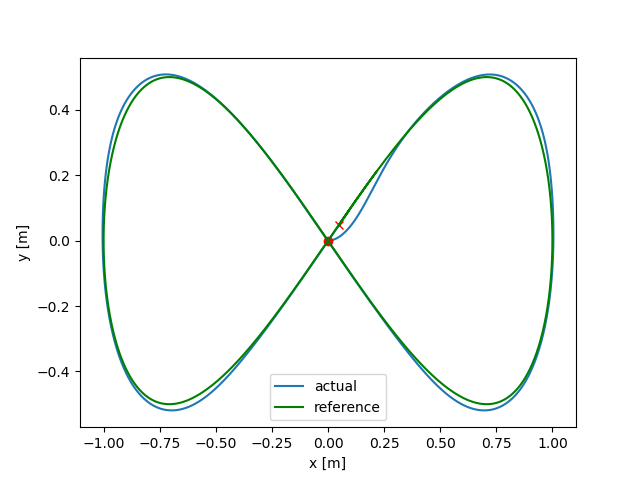
\includegraphics[scale=0.6]{kin_screenshots/Trajectory.png}
    }
    \quad
    \subfloat[Linear and angular velocities.]{
        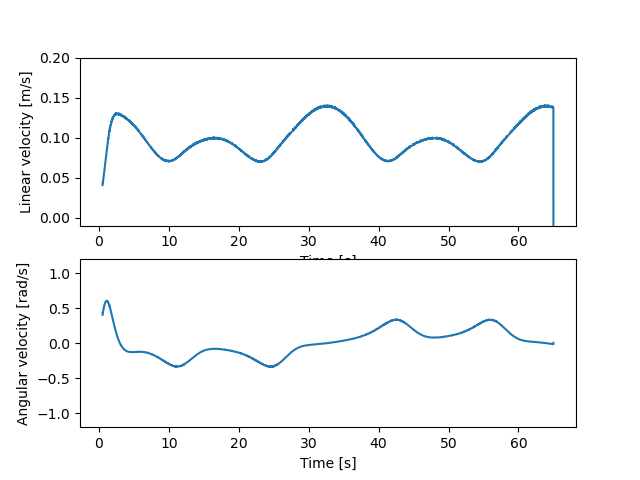
\includegraphics[scale=0.5]{kin_screenshots/Linear_and_Angular_Velocities.png}
    }
    \subfloat[Wheels velocities.]{
        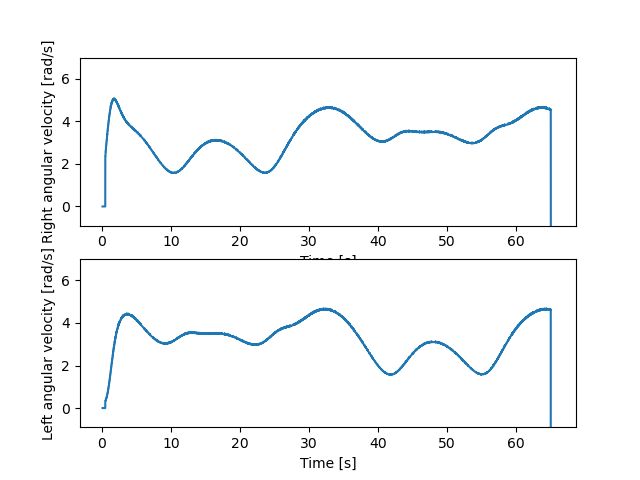
\includegraphics[scale=0.5]{kin_screenshots/Wheels_Velocities.png}
    }
    \quad
    \subfloat[Pose.]{
        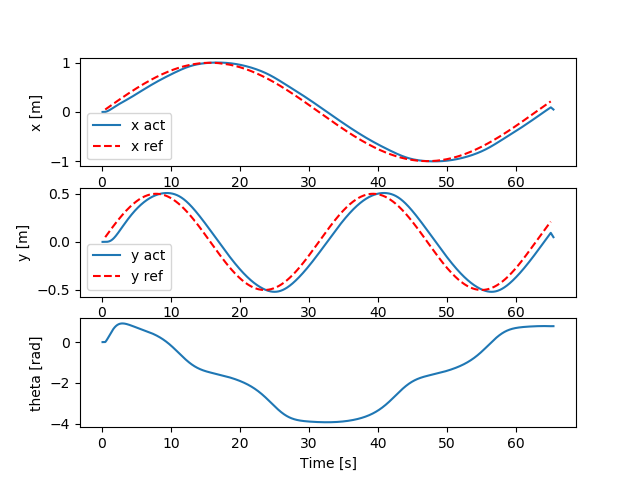
\includegraphics[scale=0.5]{kin_screenshots/Pose.png}
    }
    \subfloat[Position Error.]{
        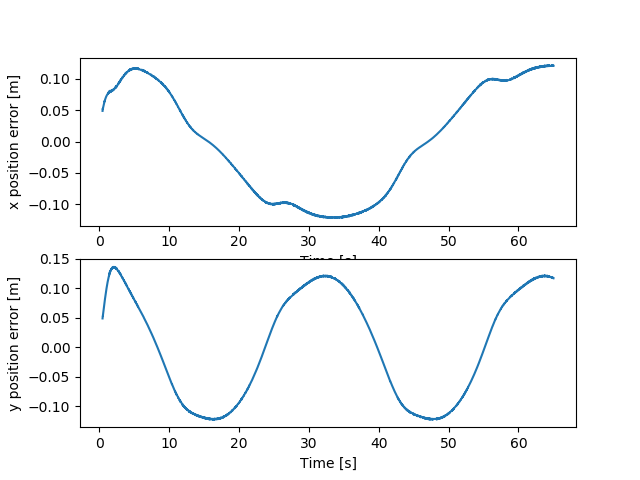
\includegraphics[scale=0.5]{kin_screenshots/Position_Error.png}
    }
    \caption[]{Behavior with the tuned custom controller.}
\end{figure}

%------------------------------------------ TUNED DWA ------------------------------------------

\subsection{Tuned DWA}

After tuning all the parameters to their optimal values, this is the final result obtained with DWA:

\begin{figure}[H]
    \centering
    \subfloat[Trajectory.]{
        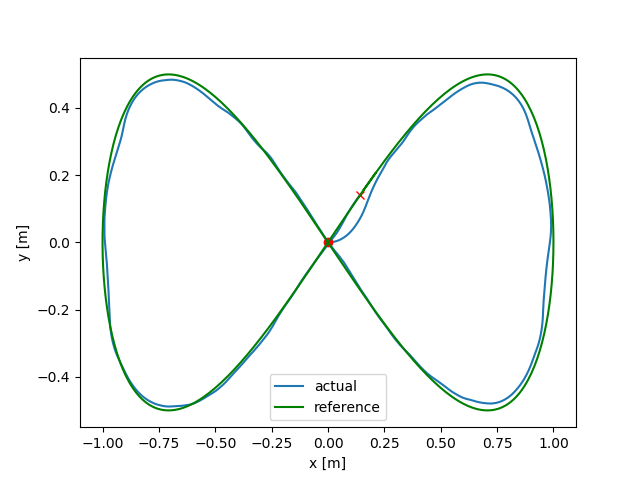
\includegraphics[scale=0.6]{dwa_screenshots/Trajectory.png}
    }
    \quad
    \subfloat[Linear and angular velocities.]{
        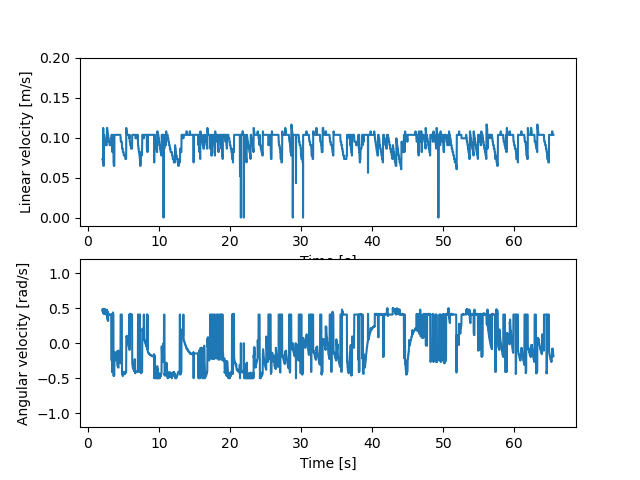
\includegraphics[scale=0.5]{dwa_screenshots/Linear_and_Angular_Velocities.png}
    }
    \subfloat[Wheels velocities.]{
        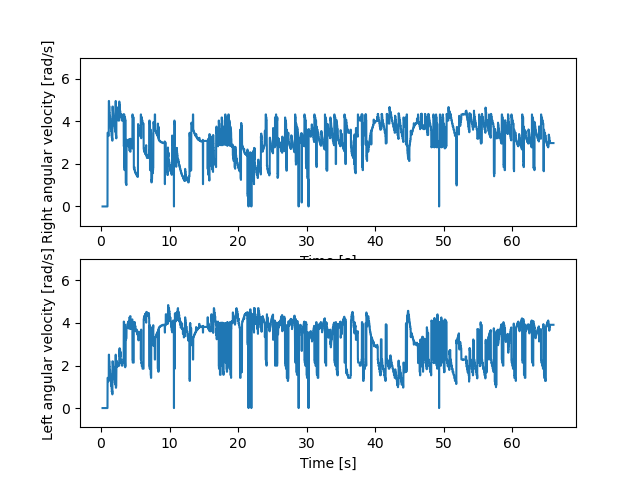
\includegraphics[scale=0.5]{dwa_screenshots/Wheels_Velocities.png}
    }
    \quad
    \subfloat[Pose.]{
        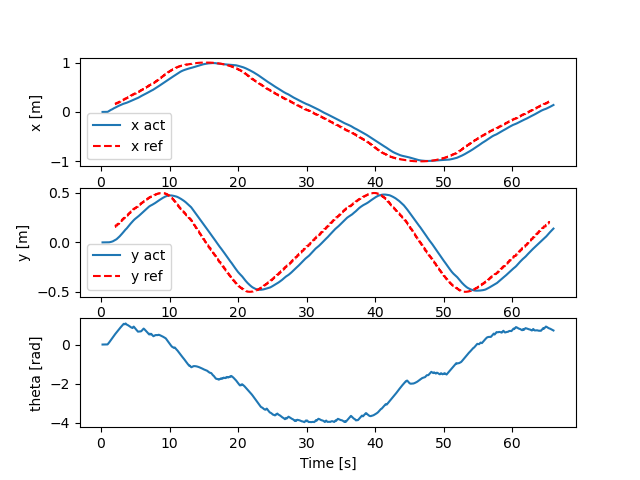
\includegraphics[scale=0.5]{dwa_screenshots/Pose.png}
    }
    \subfloat[Position Error.]{
        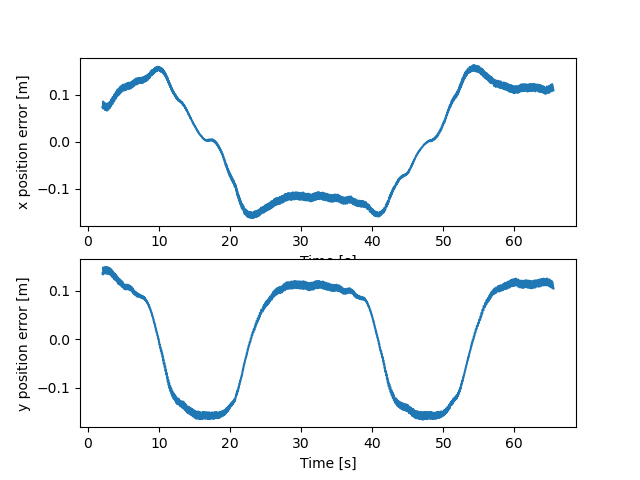
\includegraphics[scale=0.5]{dwa_screenshots/Position_Error.png}
    }
    \caption[]{Behavior with tuned DWA.}
\end{figure}

%------------------------------------------ COMPARISON ------------------------------------------

\subsection{Comparison}

Generally, the custom controller performs better than DWA due to the sudden changes (spikes) in
the velocities of the latter.
On the other hand, the performance of the two controllers is quite similar in following
the eight-shaped trajectory.

It is possible to achieve better smoothness in velocities by increasing the value
of \texttt{skipped\_goals}.
This is because when increasing the distance between two consecutive goals DWA tends to choose
a velocity closer to the current one, while the trajectory is followed in a less precise way.\\

Below there is a direct comparison between the behavior of the trajectory tracking controller and DWA.

\begin{figure}[H]
    \centering
    \subfloat[Trajectory: comparison.]{
        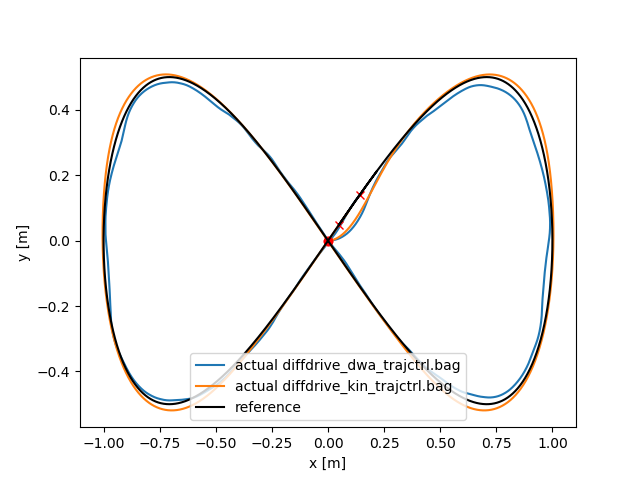
\includegraphics[scale=0.55]{comparison/Trajectory.png}
    }
    \quad
    \subfloat[Linear and angular velocities: comparison.]{
        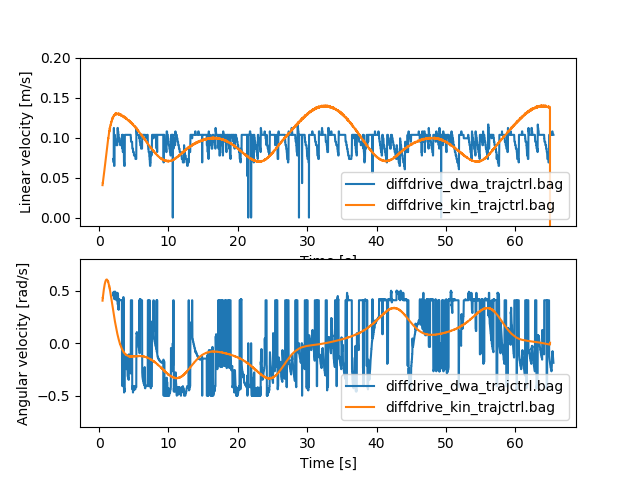
\includegraphics[scale=0.45]{comparison/Linear_and_Angular_Velocities.png}
    }
    \subfloat[Wheels velocities: comparison.]{
        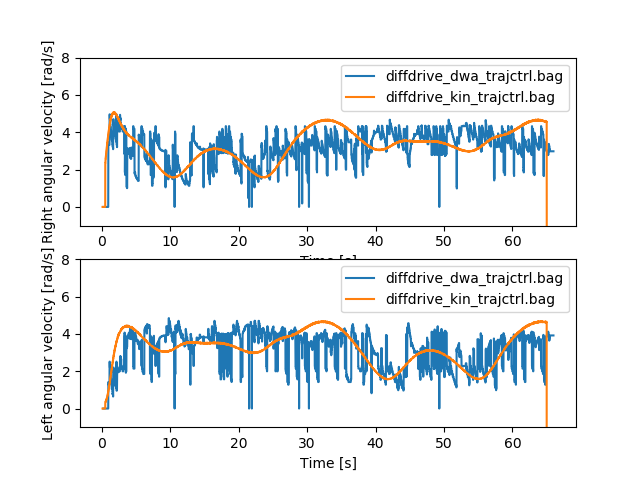
\includegraphics[scale=0.45]{comparison/Wheels_Velocities.png}
    }
    \quad
    \subfloat[Pose: comparison.]{
        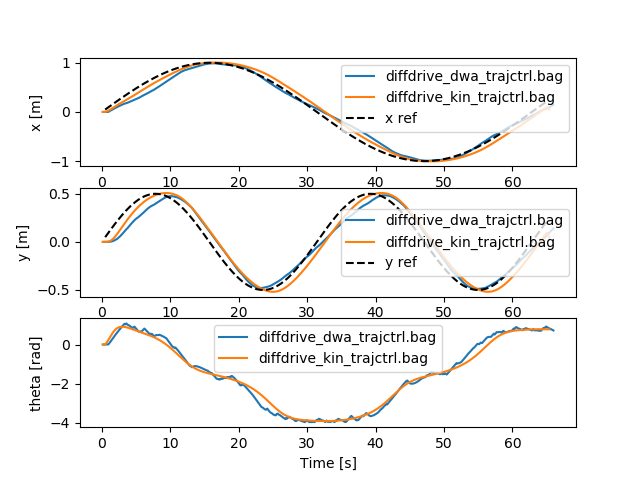
\includegraphics[scale=0.45]{comparison/Pose.png}
    }
    \subfloat[Position Error: comparison.]{
        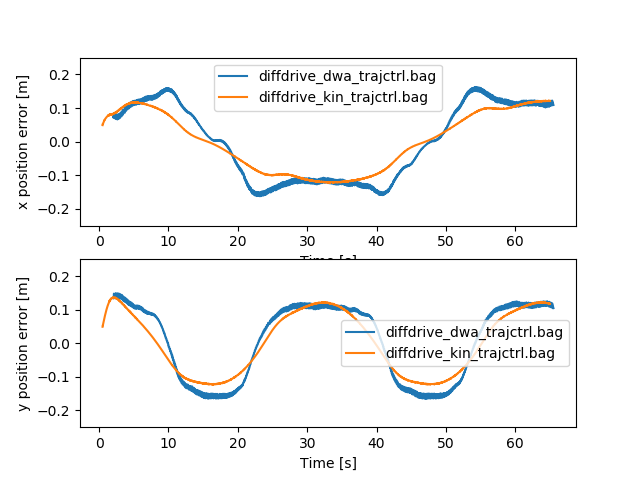
\includegraphics[scale=0.45]{comparison/Position_Error.png}
    }
    \caption[]{Comparison between the two approaches.}
\end{figure}




%--------------------------------------------------------------------------------------------------------------
%                                           ENCOUNTERED PROBLEMS
%--------------------------------------------------------------------------------------------------------------

\section{Faced issues}


%------------------------------------------ DEPRECATED PARAMETERS ------------------------------------------

\subsection{Deprecated parameters}

During the tuning phase of DWA a trial and error approach has been carried out, finding that
a few parameters are named differently in the ROS library\footnote
{\href{https://docs.ros.org/en/melodic/api/dwa\_local\_planner/html/dwa\_\_planner\_\_ros\_8cpp\_source.html}
{https://docs.ros.org/en/melodic/api/dwa\_local\_planner/html/dwa\_\_planner\_\_ros\_8cpp\_source.html}}
with respect to the ROS Wiki\footnote
{\href{https://wiki.ros.org/dwa\_local\_planner}{https://wiki.ros.org/dwa\_local\_planner}}.

Such renaming was not advertised by any error nor warning, so it was difficult to spot the root of the problem
when tuning parameters and seeing no difference in the robot's behavior.

In fact, the warning would be raised only if DWA was instantiated inside the \texttt{nav\_core} architecture,
which is not the case when using DWA standalone.\\

The following pair of parameters is an example:
\begin{itemize}
    \item \texttt{min\_rot\_vel}, which is now deprecated and has been renamed into \texttt{min\_vel\_theta};
    \item \texttt{max\_rot\_vel}, which is now deprecated and has been renamed into \texttt{max\_vel\_theta}.\\
\end{itemize}

Looking at the ROS Wiki, the parameters still have the old (wrong) name, while the source code of the library
contains some hints about the (unadvertised - outside of \texttt{nav\_core}) deprecation:

\begin{figure}[H]
    \centering
    \subfloat[ROS Wiki description.]{
        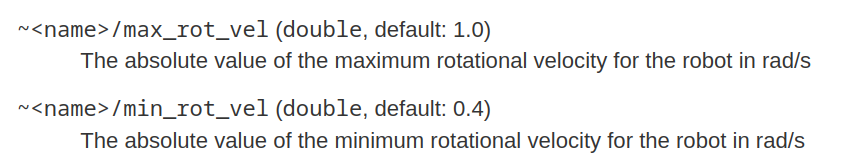
\includegraphics[scale=0.42]{other/deprecated_parameters_description.png}
    }
    \quad
    \subfloat[ROS library source code warning.]{
        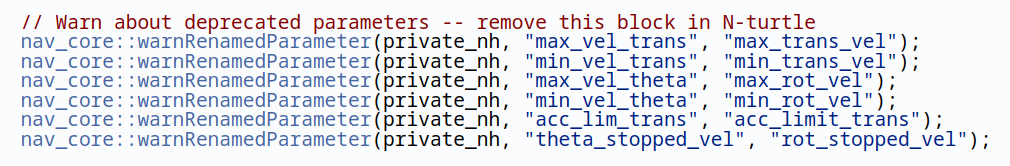
\includegraphics[scale=0.5]{other/deprecated_parameters_warning.png}
    }
    \caption[]{Deprecated parameters.}
\end{figure}


%------------------------------------------ DWA USED STANDALONE ------------------------------------------

\subsection{DWA used standalone}

Usually DWA is used inside a standard architecture which is the Navigation Stack in ROS.

However, the goal of this project is to integrate DWA in the architecture with the simulator used for
the custom controller. Thereby DWA has been rearranged in a ``standalone mode''.\\

To accomplish this, it has been necessary to provide to DWA all the information it normally expects on
certain topics, such as \texttt{/odom}, \texttt{/goal}, and \texttt{/map}.\\

Unfortunately there is no documentation for this kind of setup on the ROS Wiki, and the few lines of code
that are not working anymore due to the use of deprecated libraries (i.e. \texttt{tf} is the one mentioned
in the example, while \texttt{tf2} is the actual supported one).\\

For instance, the following snippet is the one in the ROS Wiki (not working):

\begin{lstlisting}
#include <tf/transform_listener.h>
#include <costmap_2d/costmap_2d_ros.h>
#include <dwa_local_planner/dwa_planner_ros.h>

...

tf::TransformListener tf(ros::Duration(10));
costmap_2d::Costmap2DROS costmap("my_costmap", tf);

dwa_local_planner::DWAPlannerROS dp;
dp.initialize("my_dwa_planner", &tf, &costmap);
\end{lstlisting}

Instead, the code above must be modified as follow to correctly work:

\begin{lstlisting}
#include <tf2_ros/transform_listener.h>
#include <costmap_2d/costmap_2d_ros.h>
#include <dwa_local_planner/dwa_planner_ros.h>

...

tf2_ros::Buffer tfBuffer(ros::Duration(10));
tf2_ros::TransformListener tfListener(tfBuffer);
costmap_2d::Costmap2DROS my_global_costmap("my_global_costmap", tfBuffer);
my_global_costmap.start();

dwa_local_planner::DWAPlannerROS dp;
dp.initialize("my_dwa_planner", &tfBuffer, &my_global_costmap);
\end{lstlisting}


%------------------------------------------ MULTIPLE GOALS ------------------------------------------

\subsection{Multiple goals}

In a standard scenario DWA needs only a single final goal and computes the full trajectory on its own.

In this project the trajectory is predefined and must be explicitly forced.
This is done by continuously changing the goal, otherwise the robot would go straight to the final
point of the overall eight-shaped trajectory skipping all the intermediate points.\\

The issue here is that a too dense vector of goal points would lead to an unsteady profile in
the velocities, while a too sparse vector would lead to a large deviation from the reference trajectory.

Therefore a suitable value for the density of those points must have been searched to achieve a correct behavior.




%--------------------------------------------------------------------------------------------------------------
%                                           USAGE OF THE CODE
%--------------------------------------------------------------------------------------------------------------

\section{Usage of the code}


%------------------------------------------ INSTALLATION ------------------------------------------

\subsection{Installation}

First of all, all the software written in this project has been tested on \textit{Ubuntu 18.04 LTS}
and \textit{ROS Melodic}.

For the following commands you are expected to already have Ubuntu 18.04 installed.\\

First, install ROS and all the required packages:

\begin{lstlisting}
sudo apt instal ros-melodic-desktop-full
sudo apt install ros-melodic-costmap-2d ros-melodic-base-local-planner ros-melodic-dwa-local-planner ros-melodic-map-server
\end{lstlisting}


%------------------------------------------ SETUP AND COMPILATION ------------------------------------------

\subsection{Setup and compilation}

Clone or download the repository into your home (\texttt{$\sim$/}) folder.\\

If using bash, add the following line to the end of your \texttt{$\sim$/.bashrc} file:
\begin{lstlisting}
source ~/ROS_trajectory_tracking_controller/devel/setup.bash
\end{lstlisting}

If using zsh instead, add this other line to the end of your \texttt{$\sim$/.zshrc} file:
\begin{lstlisting}
source ~/ROS_trajectory_tracking_controller/devel/setup.zsh
\end{lstlisting}

Enter the project root directory and compile everything with:
\begin{lstlisting}
cd ROS_trajectory_tracking_controller
catkin_make
\end{lstlisting}


%------------------------------------------ SIMULATION AND RESULTS ------------------------------------------

\subsection{Simulation and results}

The following instructions let you perform and visualize a simulation.

\subsubsection{Custom controller}

This simulation shows the behavior of the custom controller when an eight-shaped trajectory is set.

You will need two open terminals: one for launching the project, the other to record and plot the data.\\

\textit{[terminal 1]} Enter the \texttt{script/} folder and start recording data:
\begin{lstlisting}
cd ~/ROS_trajectory_tracking_controller/src/diffdrive_kin_ctrl/script
rosbag record -a -O diffdrive_kin_trajctrl.bag
\end{lstlisting}

\textit{[terminal 2]} Start the simulation:
\begin{lstlisting}
roslaunch diffdrive_kin_ctrl diffdrive_kin_trajctrl.launch
\end{lstlisting}

Wait until the end of the simulation (when the robot stops moving).\\

\textit{[terminal 1]} Stop the recording with Ctrl-C.\\

\textit{[terminal 2]} Stop the simulation with Ctrl-C.\\

\textit{[terminal 1]} Visualize the recorded data:
\begin{lstlisting}
python plot_results.py diffdrive_kin_trajctrl.bag
\end{lstlisting}

\subsubsection{DWA}

This simulation shows the behavior of DWA when an eight-shaped trajectory is set.

You will need two open terminals: one for launching the project, the other to record and plot the data.\\

\textit{[terminal 1]} Enter the script/ folder and start recording data:
\begin{lstlisting}
cd ~/ROS_trajectory_tracking_controller/src/diffdrive_kin_ctrl/script
rosbag record -a -O diffdrive_dwa_trajctrl.bag
\end{lstlisting}

\textit{[terminal 2]} Start the simulation:
\begin{lstlisting}
roslaunch diffdrive_dwa_ctrl diffdrive_dwa_trajctrl.launch
\end{lstlisting}

Wait until the end of the simulation (when the robot stops moving).\\

\textit{[terminal 1]} Stop the recording with Ctrl-C.\\

\textit{[terminal 2]} Stop the simulation with Ctrl-C.\\

\textit{[terminal 1]} Visualize the recorded data:
\begin{lstlisting}
python plot_results.py diffdrive_dwa_trajctrl.bag
\end{lstlisting}

\subsubsection{Compare two simulations}

If you wish, you can also compare the results of the two different simulations.\\

Given the two bag files already recorded as written above, visualize the comparison
(specify the DWA bag first):
\begin{lstlisting}
python plot_comparison.py diffdrive_dwa_trajctrl.bag diffdrive_kin_trajctrl.bag
\end{lstlisting}




%--------------------------------------------------------------------------------------------------------------
%                                               CONCLUSION
%--------------------------------------------------------------------------------------------------------------

\section{Conclusion}

The project compares two approaches to make a robot follow a predefined trajectory: a custom controller,
which uses a PID and a linearisation law, and DWA in its ROS implementation.\\

It has been shown how the two techniques behave in the particular case of following an eight-shaped trajectory
in an ideal flat map with no obstacles.
The presented results are the output of an optimal parameters configuration.
Vastly different (worse) results can be obtained by changing, even slightly, those parameters.\\

Regarding the trajectory tracking aspect only, the two methods behave in a similar way even though the custom
controller performs moderately better than DWA.
However, the most noticeable difference is in the smoothness of the plots of linear and angular velocities:
the custom controller produces velocities that are much smoother and realistic than those produced by DWA.\\

In conclusion, this project allows the user to simulate two different approaches in a quick and easy way,
while also exposing a lot of tunable parameters.
This way the user is able to try out different behaviors at the change of those parameters, which have
been extensively documented above.




\end{document}
